\documentclass[a4paper]{article}

\usepackage{cmap}%
\usepackage[LGR,T1]{fontenc}%
\usepackage[utf8]{inputenc}%
\usepackage{alphabeta}%
\usepackage[greek,english]{babel}%
\languageattribute{greek}{polutoniko}%
\usepackage{hyperref}%
\addto\extrasenglish{\def\figureautorefname{figure}}%
\usepackage{lmodern}%

\usepackage{xcolor}
\usepackage{mathtools}
\usepackage{mdframed}
\usepackage[inline]{enumitem}
\usepackage{natbib}
\usepackage{pdflscape}
\usepackage{stmaryrd}
\usepackage{comment}
\usepackage{ifthen}
\usepackage{tikz}
\usepackage{tikz-qtree}
\usepackage{textcomp}

\usepackage{amsmath, amscd, amsthm, amssymb, mathrsfs, amsfonts, wasysym}%
\let\oldemptyset\emptyset%
\let\emptyset\varnothing%
\usepackage{cancel}%

\usepackage{tabularx}%
\usepackage{multirow}%
\renewcommand{\arraystretch}{3}%

\usepackage{pict2e}
\usepackage{picture}

\newcommand{\varslash}{%
  \mathbin{\mathpalette\pictslash{{0}{1}}}%
}
\newcommand{\varbslash}{%
  \mathbin{\mathpalette\pictslash{{1}{-1}}}%
}

\makeatletter
\newcommand{\pictslash}[2]{%
  \vcenter{%
    \sbox0{$\m@th#1\varobslash$}\dimen0=.55\wd0
    \hbox to\wd 0{%
      \hfil\pictslash@aux#2\hfil
    }%
  }%
}
\newcommand{\pictslash@aux}[2]{%
    \begin{picture}(\dimen0,\dimen0)
    \roundcap
    \linethickness{.15ex}
    \put(0,#1\dimen0){\line(1,#2){\dimen0}}
    \end{picture}%
}
\makeatother

\def\downmapsto{\rotatebox[origin=c]{270}{\ensuremath{\mapsto}}}%

\usepackage{bussproofs}%
\EnableBpAbbreviations%
\def\fCenter  {\mathbin{\vdash}}%
\def\la       {\leftarrow}%
\def\ra       {\rightarrow}%
\def\impl     {\mathbin{\slash}}%
\def\impr     {\mathbin{\backslash}}%
\def\prod     {\bullet}%
\def\prodl    {\bullet}%
\def\prodr    {\bullet}%
\def\himpl    {\!\!\fatslash\:}%
\def\himpr    {\fatbslash}%
\def\hprod    {\mathbin{\circ}}%
\def\hprodl   {\mathbin{\circ}}%
\def\hprodr   {\mathbin{\circ}}%
\def\trace    {\ensuremath{\text{trace}}}%
\def\unit     {\ensuremath{\mathbf{I}}}%
\def\sq       {\ensuremath{\Box}}%
\def\di       {\ensuremath{\Diamond}}%
\def\diIfx    {\ensuremath{\hat{\di}}}%
\def\sqIfx    {\ensuremath{\hat{\sq}}}%
\def\diExt    {\rotatebox[origin=c]{180}{\diIfx}}%
\def\sqExt    {\rotatebox[origin=c]{180}{\sqIfx}}%
\def\vsep     {\ \vert\ }%
\def\e        {\ensuremath{\mathbf{e}}}%
\def\t        {\ensuremath{\mathbf{t}}}%
\def\lamET    {\ensuremath{\lambda^{\ra}_{\{\e,\t\}}}}%
\def\S        {\text{S}}%
\def\N        {\text{N}}%
\def\NP       {\text{NP}}%
\def\PP       {\text{PP}}%
\def\INF      {\text{INF}}%
\def\A        {\text{A}}%
\def\IV       {\text{IV}}%
\def\TV       {\text{TV}}%
\def\I        {\ensuremath{\mathbf{I}}}%
\def\B        {\ensuremath{\mathbf{B}}}%
\def\C        {\ensuremath{\mathbf{C}}}%
\def\john     {\ensuremath{\text{john}}}%
\def\mary     {\ensuremath{\text{mary}}}%
\def\bill     {\ensuremath{\text{bill}}}%
\def\walks    {\ensuremath{\text{walks}}}%
\def\damned   {\ensuremath{\text{damned}}}%
\def\dog      {\ensuremath{\text{dog}}}%
\def\likes    {\ensuremath{\text{likes}}}%
\def\sees     {\ensuremath{\text{sees}}}%
\def\leave    {\ensuremath{\text{leave}}}%
\def\wants    {\ensuremath{\text{wants}}}%
\def\everyone {\ensuremath{\text{everyone}}}%
\def\different{\ensuremath{\text{different}}}%
\def\someone  {\ensuremath{\text{someone}}}%
\def\served   {\ensuremath{\text{served}}}%
\def\a        {\ensuremath{\text{a}}}%
\def\waiter   {\ensuremath{\text{waiter}}}%
\def\JOHN     {\ensuremath{\mathbf{john}}}%
\def\PERSON   {\ensuremath{\mathbf{person}}}%
\def\WAITER   {\ensuremath{\mathbf{waiter}}}%
\def\WALK     {\ensuremath{\mathbf{walk}}}%
\def\LIKE     {\ensuremath{\mathbf{like}}}%
\def\SERVE    {\ensuremath{\mathbf{serve}}}%
\def\SEE      {\ensuremath{\mathbf{see}}}%
\def\DAMN     {\ensuremath{\mathbf{damn}}}%
\def\PAST     {\ensuremath{\mathbf{past}}}%
\def\DOG      {\ensuremath{\mathbf{dog}}}%
\def\WANT     {\ensuremath{\mathbf{want}}}%
\def\plug     {\ensuremath{\:\cdot\:[\:\cdot\:]}}%
\def\qdown    {\ensuremath{\mathbf{Q}{\downarrow}}}
\def\qup      {\ensuremath{\mathbf{Q}{\uparrow}}}

\newcommand{\q}       [1][{\cdot}]{\mathbf{Q}(#1)}%
\newcommand{\focus}   [1]{\boxed{#1}}%
\newcommand{\struct}  [1]{{\cdot}#1{\cdot}}%
\newcommand{\sub}     [3]{#1[#2/#3]}%
\newcommand{\tr}      [1][({\cdot})]{#1^*}%
\newcommand{\trd}     [1][({\cdot})]{#1^{**}}%
\newcommand{\case}    [4]{\text{case}\;#1\;\text{of}\;(#2, #3)\ra#4}%
\newcommand{\add}     [2]{#1 + #2}
\newcommand{\mathplus}[0]{+}

\renewcommand*{\&}{%
  \relax
  \ifmmode
    \mathbin{\char`\&}%
  \else
    \char`\&\relax
  \fi
}

\newenvironment{pfbox}[1][0.9]%
  {\gdef\scalefactor{#1} \leavevmode\hbox\bgroup}
  {\scalebox{\scalefactor}{\DisplayProof} \egroup}

\newenvironment{pfblock}[1][0.9]%
  {\gdef\scalefactor{#1}\begin{center}\proofSkipAmount \leavevmode}%
  {\scalebox{\scalefactor}{\DisplayProof}\proofSkipAmount \end{center} }

\newboolean{notes}%
\setboolean{notes}{true}%
\providecommand{\todo}[1]{%
  \ifthenelse%
  {\boolean{notes}}%
  {\textcolor{red}{\_}\marginpar{\color{red}#1}}%
  {}}
\providecommand{\note}[1]{%
  \ifthenelse%
  {\boolean{notes}}%
  {{\color{green}\textbf{NOTE:~}#1}}%
  {}}


% rules from the Haskell code
\newcommand{\AxR}[1]{\AXC{}\RightLabel{Ax$^L$}\UIC{$#1$}}%
\newcommand{\AxL}[1]{\AXC{}\RightLabel{Ax$^R$}\UIC{$#1$}}%
\newcommand{\UnfR}[1]{\RightLabel{Foc$^R'$}\UIC{$#1$}}%
\newcommand{\UnfL}[1]{\RightLabel{Foc$^L'$}\UIC{$#1$}}%
\newcommand{\FocR}[1]{\RightLabel{Foc$^R$}\UIC{$#1$}}%
\newcommand{\FocL}[1]{\RightLabel{Foc$^L$}\UIC{$#1$}}%
\newcommand{\WithL}[2]{\RightLabel{\&L$_{#1}$}\UIC{$#2$}}%
\newcommand{\WithR}[1]{\RightLabel{\&R}\BIC{$#1$}}%
\newcommand{\ImpRL}[1]{\RightLabel{$\impr$L}\BIC{$#1$}}%
\newcommand{\ImpRR}[1]{\RightLabel{$\impr$R}\UIC{$#1$}}%
\newcommand{\ImpLL}[1]{\RightLabel{$\impl$L}\BIC{$#1$}}%
\newcommand{\ImpLR}[1]{\RightLabel{$\impl$R}\UIC{$#1$}}%
\newcommand{\Res}[3]{%
  \RightLabel{%
    \ifstrequal{1}{#1}{%
      \ifstrequal{1}{#2}{%
        Res$\impr\prod$ % Res11
      }{%
        \ifstrequal{2}{#2}{%
          Res$\prod\impr$ % Res12
        }{%
          \ifstrequal{2}{#2}{%
            Res$\impl\prod$ % Res13
          }{%
            Res$\prod\impl$ % Res14
          }
        }
      }
    }{%
      \ifstrequal{1}{#2}{%
        Res$\sq\di$ % Res21
      }{%
        Res$\di\sq$ % Res22
      }
    }
  }
  \UIC{$#3$}
}%
\newcommand{\DiaL}[1]{\RightLabel{$\di$L}\UIC{$#1$}}%
\newcommand{\DiaR}[1]{\RightLabel{$\di$R}\UIC{$#1$}}%
\newcommand{\BoxL}[1]{\RightLabel{$\sq$L}\UIC{$#1$}}%
\newcommand{\BoxR}[1]{\RightLabel{$\sq$R}\UIC{$#1$}}%
\newcommand{\IfxRR}[1]{\RightLabel{$\Ifx$RR}\UIC{$#1$}}%
\newcommand{\IfxLR}[1]{\RightLabel{$\Ifx$LR}\UIC{$#1$}}%
\newcommand{\IfxLL}[1]{\RightLabel{$\Ifx$LL}\UIC{$#1$}}%
\newcommand{\IfxRL}[1]{\RightLabel{$\Ifx$RL}\UIC{$#1$}}%
\newcommand{\ExtRR}[1]{\RightLabel{$\Ext$RR}\UIC{$#1$}}%
\newcommand{\ExtLR}[1]{\RightLabel{$\Ext$LR}\UIC{$#1$}}%
\newcommand{\ExtLL}[1]{\RightLabel{$\Ext$LL}\UIC{$#1$}}%
\newcommand{\ExtRL}[1]{\RightLabel{$\Ext$RL}\UIC{$#1$}}%
\newcommand{\UnitRL}[1]{\RightLabel{$\I$L}\UIC{$#1$}}%
\newcommand{\UnitRR}[1]{\RightLabel{$\I$R}\UIC{$#1$}}%
\newcommand{\UnitRI}[1]{\RightLabel{$\I^-$}\UIC{$#1$}}%
\newcommand{\DnB}[1]{\RightLabel{$\B$}\UIC{$#1$}}%
\newcommand{\UpB}[1]{\RightLabel{$\B'$}\UIC{$#1$}}%
\newcommand{\DnC}[1]{\RightLabel{$\C$}\UIC{$#1$}}%
\newcommand{\UpC}[1]{\RightLabel{$\C'$}\UIC{$#1$}}%

\ifdefined\usetheme\usetheme{Boadilla}\fi
\ifdefined\usecolortheme\usecolortheme{seagull}\fi
\ifdefined\beamertemplatenavigationsymbolsempty\beamertemplatenavigationsymbolsempty\fi


\begin{document}

% ``We are constructing a \emph{grammar logic}. Therefore, we only
% want features in our logic for which we can demonstrate a motivating
% example from natural language.''

% - implicit semantic calculus;
% - explicit semantic calculus;
% - syntactic calculus;
% - display calculus;
% - compositionality principle;
% - problems with compositionality;
% - quantifier raising and scope ambiguity;
% - continuation monad & delimited continuations;
% - extension: lexical ambiguity;
% - extension: quantifier raising
%   * treatment of some & every;
%   * treatment of same & different;
%   * treatment of plurals;
% - extension: scope islands;

\section{Introduction}
\label{sec:introduction}

In this thesis, I will discuss the grammar logic NLQ, an extension of
the non-associative Lambek calculus, which is capable of analysing
quantifier movement, scope islands, infixation and extraction.

% This thesis is not meant to be a work of thorough linguistic
% analysis.
What I hope to do in this thesis is to \emph{extend} and
\emph{solidify} the logical vocabulary with which such linguistic
analyses can be made. In this, I will use the following guiding
principles:
\begin{itemize}
\item We are constructing a \emph{grammar} logic. Therefore, we only
  want features in our logic for which we can demonstrate a motivating
  example from natural language.
\item We are constructing a grammar \emph{logic}. Therefore, we will
  only accept extensions to our logic if we can show that they
  preserve our most important properties: we want our logic to be
  reflexive and transitive, and want a procedure for proof
  search that is both \emph{decidable} and \emph{complete}.
\end{itemize}
I am under no impression that the extensions I am proposing will be
the be-all and end-all of logical grammar, so another important point
in this thesis will be \emph{modularity}.
It is incredibly important to formulate extensions in a modular
manner, so that other logical grammarians are free to mix and
match extensions without having to worry about unforeseen
interactions. There are two key techniques for this:
\begin{enumerate*}[label=(\arabic*)]
\item
  we use display calculus to get a general procedure for
  cut-elimination (\autoref{sec:display-calculus}); and
\item
  we associate each syntactic extension with its own set of
  connectives (or \emph{modality}) and make sure that the inference
  rules in that extension only apply in the presence of these
  connectives (\autoref{sec:syntactic-approaches-to-scope}).
\end{enumerate*}

Another key point will be \emph{unique normal-forms}---in our proof
search procedure, we only want to find a single proof for each
interpretation that a sentence has. In our calculus, we will achieve
this using \emph{focusing}
(\autoref{sec:focusing-and-spurious-ambiguity}).

The last key point in this thesis will be \emph{verification}. It is
far too easy to make mistakes when writing down logical proofs in a
pen-and-paper style, or when manually typesetting them in
\LaTeX. Therefore, most of the claims I make in this thesis will be
backed up by a pair of verified implementations of the full version
of NLQ (i.e. the version using all discussed extensions).
These verifications can be found in appendices A and B and on GitHub.

In appendix A, we discuss a formalisation in Agda \citep{norell2009}.
We implement the grammar logic, prove some key properties, and give a
formal semantics in the form of a translation from proofs in NLQ to
Agda terms.

In appendix B, we discuss a formalisation in Haskell
\citep{marlow2010} using the singletons library
\citet{eisenberg2012}. In the full version, we implement the grammar
logic, implement proof search, and give a formal semantics in the form
of a translation into a subset of Haskell which includes meaning
postulates. However, because the implementations of the grammar logic
are nearly identical, we restrict our discussion of the Haskell
version to the interface provided by the library, and how to write
your own lexicon and example sentences.

Starting in \autoref{sec:what-is-type-logical-grammar}, we will give a
brief introduction to type-logical grammar in general, and to what I
consider to be the base type-logical grammar: the non-associative
Lambek calculus (NL) paired with a simple semantic lambda calculus
(\lamET).
In \autoref{sec:display-calculus}, we will discuss the display
calculus formulation of NL, and motivate our usage of display
calculus.
Then, in sections \ref{sec:lexical-ambiguity} and
\ref{sec:movement-and-quantifier-raising}, we will discuss several
extension to the base type-logical grammar.

\subsection{What is type-logical grammar?}
\label{sec:what-is-type-logical-grammar}

Before we address the question of what type-logical grammar is, let us
try and get an idea of what problem it is trying to solve. Have a look
at the abstract pipeline for natural language understanding (NLU) in
\autoref{fig:abstract-nlu-pipeline}.

\begin{figure}[hb]
  \begin{mdframed}
    \centering
    \begin{minipage}{0.35\linewidth}%
      \centering
      \framebox{Morphological}\\
      $\downarrow$\\
      \framebox{Lexical}\\
      $\downarrow$\\
      \framebox{Syntactic}\\
      $\downarrow$\\
      \framebox{Semantic}\\
      $\downarrow$\\
      \framebox{Pragmatic}\\
    \end{minipage}
    \begin{minipage}{0.55\linewidth}%
      \centering
      ``Mary saw foxes.''\\
      $\downarrow$\\
      Mary see.PAST fox.PL\\
      $\downarrow$\\
      Mary:NP see:TV.PAST fox:NP.PL\\
      $\downarrow$\\
      Mary:NP [see:TV.PAST fox:NP.PL]\\
      $\downarrow$\\
      $\exists X. X \subseteq\mathbf{fox}\land\mathbf{past}(\mathbf{see}(\text{Mary},X))$\\
      $\downarrow$\\
      \ldots\footnotemark\\
    \end{minipage}
  \end{mdframed}
  \caption{An abstract pipeline for natural language
    understanding.}%
  \label{fig:abstract-nlu-pipeline}
\end{figure}%
\footnotetext{%
  As the pragmatic function is all about integrating context (be it
  textual or environmental) into the meaning, it would not make sense
  to list something here.
}


To the left of the figure, you see the various phases or functions
commonly associated with an NLU-pipeline. To the right, you see the
inputs and outputs of these functions.
For instance, the morphological function will take an unanalysed
sentence, and return a sentence which is lemmatised. This entails that
all morphemes are made explicit---for instance, in the case of the
example in \autoref{fig:abstract-nlu-pipeline}, the previously
``implicit'' morphemes for past tense and plurality are added.

There is some disagreement on the exact role of type-logical grammars in
this pipeline. Ideally, type-logical grammars would play the role of
both the syntactic and the semantic function. However, the current
state of affairs in research is that often only the semantic function
is truly considered\footnote{%
  This statement is not true for \emph{associative} type-logical
  grammars, which fundamentally reject the tree structure of
  language---that is, they assume that the meaning of a sentence
  depends solely on the linear order of words, and not on some hidden
  tree structure.
}. This makes sense from a research perspective: we can refer to the
huge body of work on generative grammar to inform our choice for
sentence structure, and focus on assigning the right meaning to these
structures. This is also the approach we will also take in this
thesis---that is, we consider type-logical grammars to be the
function:
\begin{center}
  Mary:NP [see:TV.PAST fox:NP.PL]\\
  $\downarrow$\\
  \framebox{Type-Logical Grammar}\\
  $\downarrow$\\
  $\exists X.X\subseteq\mathbf{fox}\land\mathbf{past}(\mathbf{see}(\text{mary},X))$
\end{center}
That is, it is a function which, given some structured and typed input
which represents the syntactic structure of a sentence, returns the
meaning(s) associated with that sentence.

Given the presence of the phrase ``structured and typed'', we may
already suspect that type theory offers a fitting solution to this
problem. And indeed, under the guise of type-logical grammar, it
does. A type-logical grammar generally consists of three things:
\begin{enumerate}[label=(\arabic*)]
\item a syntactic calculus, set up in such a fashion that only
  grammatical sentences are well-typed, and for which an efficiently
  decidable procedure for proof-search exists;
\item a semantic calculus, used to represent the meanings of words and
  sentences; and
\item a translation from the syntactic to the semantic calculus.
\end{enumerate}
We interpret the part-of-speech tags in our input (NP, TV, etc.) as
types in the syntactic calculus, and combine these with the desired
type for the tree---usually \S\ for `sentence'---to form an input
sequent.
We then search for a proof of that sequent in the syntactic calculus,
and translate it to a term in the semantic calculus.
Once there, we interpret the morphemes (e.g.\ lemmas, \texttt{PAST},
\texttt{PL}, etc.) as terms in the semantic calculus.

In \autoref{sec:simple-type-logical-grammar}, we will have a look at
the base type-logical grammar, and give some examples of the process
of deriving sentence meaning.



\subsection{A simple type-logical grammar}
\label{sec:simple-type-logical-grammar}

The simplest type-logical grammar that comes to mind---drawing
heavily from Montague grammar and categorial grammar---is composed of
the simply-typed lambda calculus with atomic types \e\ and \t\ (\lamET) as
a semantic calculus, and the non-associative Lambek calculus
\citep[NL;][]{lambek1961} as a syntactic calculus.

The usual natural deduction formulation of \lamET\ can to be seen in
\autoref{fig:implicit-lamET}. It is a simple lambda
calculus, with atomic types \e\ (`entity') and \t\ (`truth-value').
In addition, we usually assume that any logical operator or
word-meanings we need is defined as a constant of the appropriate
type. For instance, $\forall$ is a constant of type $(\e\ra\t)\ra\t$,
and `john' is a constant of type \e. Note that we will sometimes write
logical operators in their usual notation, e.g.\ $M\wedge N$ or
$\forall x.M$, but this should be taken as syntactic sugar, in the
case of our examples rewriting to $(({\wedge}\;M)\;N)$ and
$\forall\;(\lambda{x}.M)$, respectively. Additionally, we will
occasionally write e.g.\ $\e\e\t$ instead of $\e\ra\e\ra\t$, or
$(\e\t)\t$ instead of $(\e\ra\t)\ra\t$, using adjacency to mean
implication.

\begin{figure}[h]
  \begin{mdframed}
    \centering
    \begin{alignat*}{4}
      \text{Atom}       \;&α  &&\coloneqq \e\vsep\t\\
      \text{Type}       \;&A,B&&\coloneqq α\vsep A\ra B\\
      \text{Term}       \;&M,N&&\coloneqq x\vsep C\vsep\lambda x.M\vsep(M\;N)\\
      \text{Constant}   \;&C  &&\coloneqq
      {\forall}\vsep{\exists}\vsep{\neg}\vsep{\supset}\vsep{\land}\vsep{\lor}\vsep\ldots\\
      \text{Environment}\;&Γ  &&\text{set of typing assumptions of the form `$M : A$'}
    \end{alignat*}

    \begin{pfbox}
      \AXC{$(x : A)\in Γ$} \RightLabel{{Ax}} \UIC{$Γ\fCenter x : A$}
    \end{pfbox}
    \\[1\baselineskip]
    \begin{pfbox}
      \AXC{$Γ,x : A\fCenter M : B$} \RightLabel{$\ra${I}}
      \UIC{$Γ\fCenter \lambda x.M : A\ra B$}
    \end{pfbox}
    \begin{pfbox}
      \AXC{$Γ\fCenter M : A\ra B$} \AXC{$Γ\fCenter N : A$}
      \RightLabel{$\ra${E}} \BIC{$Γ\fCenter (M\;N) : B$}
    \end{pfbox}

    \todo{Reference to Montague?}

    \vspace*{1\baselineskip}
  \end{mdframed}
  \caption{\lamET, a simple semantic calculus.}%
  \label{fig:implicit-lamET}
\end{figure}
%

Using this calculus as a semantics function directly would
over-generate, e.g.\ for the sequent $\{\text{john}:\e,
\text{likes}:\e\ra\e\ra\t, \text{mary}:\e\}\fCenter\t$ we can derive
$((\text{likes}\; \text{john})\; \text{mary})$, $((\text{likes}\;
\text{mary})\; \text{john})$, $((\text{likes}\; \text{mary})\;
\text{mary})$ and $((\text{likes}\; \text{john})\; \text{john})$.
The reason for this is, of course, that the set structure used in this
formulation is much too expressive for natural language grammar.

If we want more control over the structure of our terms, a good first
step is to move to a purely syntactic formulation, where all the
structural properties are made explicit in the calculus itself; this
has been done in \autoref{fig:explicit-lamET}. We have
replaced the set by a (possibly empty) binary tree, spanned by the
structural product `$\prod$'. We have also included a number of new
structural rules, which implement the structure of a set: $\emptyset$E
and $\emptyset$I allow us to have an empty antecedent; contraction and
weakening tell us that we can use formulas multiple times or not at
all; and with commutativity and associativity we can change the order
of the formulas any way we like.

\begin{figure}[h]
  \begin{mdframed}
    \centering
    \begin{minipage}{0.6\linewidth}
      \begin{alignat*}{4}
        \text{Atom}     \;&α    &&\coloneqq \e\vsep\t\\
        \text{Type}     \;&A,B  &&\coloneqq α\vsep A\ra B\\
        \text{Structure}\;&Γ,Δ,Π&&\coloneqq A\vsep\emptyset\vsep Γ\prod Δ\\
        \text{Context}  \;&Σ    &&\coloneqq \Box\vsep Σ\prodl Δ\vsep Γ\prodr Σ
      \end{alignat*}
    \end{minipage}%
    \begin{minipage}{0.4\linewidth}
      \begin{align*}
        \Box [Γ]&\mapsto Γ\\
        (Σ\prodl Δ)[Γ]&\mapsto (Σ[Γ]\prod Δ)\\
        (Δ\prodr Σ)[Γ]&\mapsto (Δ\prod Σ[Γ])
      \end{align*}
    \end{minipage}

    \vspace*{\baselineskip}
    \begin{pfbox}
      \AXC{}\RightLabel{{Ax}}\UIC{$A\fCenter A$}
    \end{pfbox}

    \vspace*{\baselineskip}
    \begin{pfbox}
      \AXC{$Γ\prod A\fCenter B$}
      \RightLabel{$\ra${I}}
      \UIC{$Γ\fCenter A\ra B$}
    \end{pfbox}
    \begin{pfbox}
      \AXC{$Γ\fCenter A\ra B$}
      \AXC{$Δ\fCenter A$}
      \RightLabel{$\ra${E}}
      \BIC{$Γ\prod Δ\fCenter B$}
    \end{pfbox}

    \vspace*{\baselineskip}
    \begin{pfbox}
      \AXC{$Σ[Γ\prod \emptyset]\fCenter B$}
      \RightLabel{$\emptyset${E}}
      \UIC{$Σ[Γ]\fCenter B$}
    \end{pfbox}
    \begin{pfbox}
      \AXC{$Σ[Γ]\fCenter B$}
      \RightLabel{$\emptyset${I}}
      \UIC{$Σ[Γ\prod \emptyset]\fCenter B$}
    \end{pfbox}

    \vspace*{\baselineskip}
    \begin{pfbox}
      \AXC{$Σ[A\prod A]\fCenter B$}
      \RightLabel{Cont.}
      \UIC{$Σ[A]\fCenter B$}
    \end{pfbox}
    \begin{pfbox}
      \AXC{$Σ[Γ]\fCenter B$}
      \RightLabel{Weak.}
      \UIC{$Σ[Γ\prod A]\fCenter B$}
    \end{pfbox}

    \vspace*{\baselineskip}
    \begin{pfbox}
      \AXC{$Σ[Δ\prod Γ]\fCenter B$}
      \RightLabel{Comm.}
      \UIC{$Σ[Γ\prod Δ]\fCenter B$}
    \end{pfbox}
    \begin{pfbox}
      \AXC{$Σ[(Γ\prod Δ)\prod Π]\fCenter B$}
      \doubleLine\RightLabel{Ass.}
      \UIC{$Σ[Γ\prod (Δ\prod Π)]\fCenter B$}
    \end{pfbox}
    \vspace*{\baselineskip}
  \end{mdframed}
  \caption{\lamET, with explicit structural rules.}%
  \label{fig:explicit-lamET}
\end{figure}
%
%%% Local Variables:
%%% mode: latex
%%% TeX-master: t
%%% End:


Note that, in order to define these structural rules, we had to define
the notion of a `context'---a structure with \emph{exactly one} hole
in it---and a plugging function `\plug'---a function which inserts a
structure into that hole. The reason for this is that we have to be
able to apply commutativity and associativity \emph{anywhere} in the
structure to be able to freely change the order (and
bracketing).\footnote{%
  The contexts are not strictly necessary for $\emptyset$E,
  contraction and weakening, since we can already move any formula
  anywhere we want, but they make the proof system much more usable
  and greatly decrease the length of proofs that need to use any of
  these structural rules.
}

It is not hard to convince yourself that the implicit and explicit
versions of \lamET\ are equivalent---though we will refrain from
giving the full proof here.
Because of this equivalence, we can use the term language from
\autoref{fig:implicit-lamET} for the explicit version of
\lamET.
The term labelling of the logical rules is exactly the same. The
structural rules only manipulate structures, and therefore do not
change the terms. The only exception to this is contraction, for which
the term labelling is as follows:
\begin{prooftree}
  \AXC{$Σ[y : A\prod z : A]\fCenter M : B$}
  \RightLabel{Cont.}
  \UIC{$Σ[x : A]\fCenter M[x/y][x/z] : B$}
\end{prooftree}
Contraction takes a term with two variables of the same type, and
contracts them using substitution, which is defined as usual:
\begin{alignat*}{3}
  &x             &&[N/y] \mapsto
  \begin{cases}
    N, &\text{if}\;x=y\\
    x, &\text{otherwise}
  \end{cases}
  \\
  &C             &&[N/y] \mapsto C\\
  &(\lambda x.M) &&[N/y] \mapsto
  \begin{cases}
    \lambda x.M[N/y], &\text{if}\;x=y\\
    \lambda x.M,      &\text{otherwise}
  \end{cases}
  \\
  &(M\;M')       &&[N/y] \mapsto (M[N/y]\;M'[N/y])
\end{alignat*}

Using our explicit semantic calculus, we can construct our syntactic
calculus in three simple steps:
\begin{enumerate}
\item%
  we drop \emph{all} structural rules;
\item%
  since the implication `$\ra$' can now only take arguments directly
  from the left, we add a second implication `$\la$' which can only
  take arguments from the right---by convention, implications in this
  system are written as `$\impr$' and `$\impl$' (pronounced ``under''
  and ``over'') with the argument type written \emph{under} the slash;
\item%
  we replace the atomic semantic types \e\ and \t\ by atomic syntactic
  types, reminiscent of part-of-speech tags---in this case, we will
  use S (`sentence'), NP (`noun phrase'), N (`noun'), PP
  (`prepositional phrase') and INF (`infinitive');
\end{enumerate}
The resulting system can be seen in \autoref{fig:nl-natural-deduction},
defined along with some definitions for common part-of-speech tags,
i.e.\ \A\ (`adjective'), \IV\ (`intransitive verb') and \TV\
(`transitive verb').

\begin{figure}[h]
  \begin{mdframed}
    \centering
    \begin{minipage}{0.66\linewidth}
      \begin{alignat*}{4}
        \text{Atom}     \;&α  &&\coloneqq \S\vsep\N\vsep\NP\vsep\INF\\
        \text{Type}     \;&A,B&&\coloneqq α\vsep A\impr B\vsep B\impl A\\
        \text{Structure}\;&Γ,Δ&&\coloneqq A\vsep Γ\prod Δ
      \end{alignat*}
    \end{minipage}%
    \begin{minipage}{0.33\linewidth}
      \begin{alignat*}{3}
        &\A \;&&\coloneqq \N\impl\N\\
        &\IV\;&&\coloneqq \NP\impr\S\\
        &\TV\;&&\coloneqq \IV\impl\NP
      \end{alignat*}
    \end{minipage}
    \\[1\baselineskip]
    \begin{pfbox}
      \AXC{} \RightLabel{{Ax}} \UIC{$A\fCenter A$}
    \end{pfbox}
    \\[1\baselineskip]
    \begin{pfbox}
      \AXC{$A\prodΓ\fCenter B$} \RightLabel{$\impr${I}}
      \UIC{$Γ\fCenter A\impr B$}
    \end{pfbox}
    \begin{pfbox}
      \AXC{$Γ\fCenter A$} \AXC{$Δ\fCenter A\impr B$} \RightLabel{$\impr${E}}
      \BIC{$Γ\prodΔ\fCenter B$}
    \end{pfbox}
    \\[1\baselineskip]
    \begin{pfbox}
      \AXC{$Γ\prod A\fCenter B$} \RightLabel{$\impl${I}}
      \UIC{$Γ\fCenter B\impl A$}
    \end{pfbox}
    \begin{pfbox}
      \AXC{$Γ\fCenter B\impl A$} \AXC{$Δ\fCenter A$} \RightLabel{$\impl${E}}
      \BIC{$Γ\prod Δ\fCenter B$}
    \end{pfbox}
    \vspace*{1\baselineskip}
  \end{mdframed}
  \caption{NL \citep{lambek1961} in natural deduction style.}%
  \label{fig:nl-natural-deduction}
\end{figure}
%
\begin{figure}[h]
  \begin{mdframed}
    \begin{minipage}{0.333\linewidth}
      \begin{alignat*}{4}
        &\tr[\S]         &&\mapsto\t              \\
        &\tr[\N]         &&\mapsto\e\ra\t         \\
        &\tr[\NP]        &&\mapsto\e              \\
        &\tr[\INF]       &&\mapsto\e\ra\t         \\
        &\tr[(A\impr B)] &&\mapsto\tr[A]\ra\tr[B] \\
        &\tr[(B\impl A)] &&\mapsto\tr[A]\ra\tr[B]
      \end{alignat*}
    \end{minipage}%
    \begin{minipage}{0.666\linewidth}
      \vspace*{1\baselineskip}
      \begin{prooftree}
        \AXC{}\RightLabel{Ax}\UIC{$x:A\fCenter x:A$}
      \end{prooftree}
      \begin{prooftree}
        \AXC{$x:A\prod Γ\fCenter M:B$}
        \RightLabel{$\impr$I}
        \UIC{$Γ\fCenter \lambda x.M:A\impr B$}
      \end{prooftree}
      \begin{prooftree}
        \AXC{$Γ\fCenter N:A$}
        \AXC{$Δ\fCenter M:A\impr B$}
        \RightLabel{$\impr$E}
        \BIC{$Γ\prod Δ\fCenter (M\;N):B$}
      \end{prooftree}
      \begin{prooftree}
        \AXC{$Γ\prod x:A\fCenter M:B$}
        \RightLabel{$\impl$I}
        \UIC{$Γ\fCenter \lambda x.M:B\impl A$}
      \end{prooftree}
      \begin{prooftree}
        \AXC{$Γ\fCenter M:B\impl A$}
        \AXC{$Δ\fCenter N:A$}
        \RightLabel{$\impl${E}}
        \BIC{$Γ\prod Δ\fCenter (M\;N):B$}
      \end{prooftree}
    \end{minipage}
    \vspace*{1\baselineskip}
  \end{mdframed}
  \caption{NL (\autoref{fig:nl-natural-deduction}) with term
    labelling in \lamET\ (\autoref{fig:implicit-lamET}).}%
  \label{fig:nl-natural-deduction-to-lamET}
\end{figure}


Dropping \emph{all} structural rules may seem unnecessary, but there
is a good motivation for each rule.  For example, in the presence of
commutativity, there is no way to distinguish between ``Mary walks''
and ``walks Mary''; under weakening, we can add any word anywhere in a
grammatical sentence, and the sentence will remain grammatical---
e.g.\ ``Mary banana walks''; and with contraction, we can remove
consecutive words with the same type---which means that ``John read
a fantastic blue book'' could be taken to mean the same thing as
``John read a blue book''.

With respect to associativity, \citet[][p.\ 167]{lambek1961} mentions
that ``the most natural assignments of types to English words [would]
admit many pseudo-sentences as grammatical, e.g.\ %
\begin{center}
  (*)~\itshape John is poor sad. John likes poor him. Who works and
  John rests?
\end{center}
More examples, including specific derivations, of ungrammatical
sentences that would be admitted in the presence of associativity and
the empty structure can be found in \citet[p.\ 33, 105-106]{moot2012}.

Note that we use the product-free version of NL. The reason for this
is that we have no use for the product in this thesis. Should you need
the product, however, it is very easily added:
\begin{center}
  \begin{pfbox}
    \AXC{$\Gamma\fCenter{A}$}
    \AXC{$\Delta\fCenter{B}$}
    \RightLabel{L$\otimes$}
    \BIC{$\Gamma\prod\Delta\fCenter{A\otimes{B}}$}
  \end{pfbox}
  \begin{pfbox}
    \AXC{$\Gamma\fCenter{A\otimes{B}}$}
    \AXC{$\Sigma[A\prod{B}]\fCenter{C}$}
    \RightLabel{R$\otimes$}
    \BIC{$\Sigma[\Gamma]\fCenter{C}$}
  \end{pfbox}
\end{center}

The last component we need for our simple type-logical grammar is a
translation from our syntactic calculus to our semantic calculus,
which consists of:
\begin{enumerate}[label=(\arabic*)]
\item
  a function $\tr$, translating the types in NL to types in \lamET; and
\item
  a set of rewrite rules, that rewrite proofs in NL to proofs in \lamET.
\end{enumerate}
However, in the interest of brevity, we will often give this second
translation directly as a term labelling. For instance, in
\autoref{fig:nl-natural-deduction-to-lamET}, we give the
translation on terms by directly labelling the rules of the syntactic
calculus with semantic terms. Because there is a one-to-one
correspondence between lambda terms and proofs, this is perfectly
unambiguous.

Note that we have chosen the particular translation for atomic types
in \autoref{fig:nl-natural-deduction-to-lamET} because it
aligns well with the remainder of this thesis. However, there are
different ways to define this translation---most notably,
\citepos{montague1973} worst-case generalisation for NPs, which
interprets them as having the type $(\e\t)\t$.

Now that we have a full type-logical grammar, let's give an example
analysis of the sentence ``Mary likes Bill''. We assume the
morphological, lexical and syntactic phases have been taken care of,
which leaves us with the following endsequent:
\[
  \text{mary}:\NP\prod(\text{likes}:\TV\prod\text{bill}:\NP)\;\fCenter\;?:\S
\]
Fortunately, proof search is decidable for this system, so we can
simply search the space of all possible proofs of this sequent. As it
turns out, the only proof is:
\begin{center}
  \vspace*{-1\baselineskip}
  \begin{pfbox}[0.8]
    \AXC{}\RightLabel{Ax}\UIC{$\text{mary}:\NP\fCenter\text{mary}:\NP$}
    \AXC{}\RightLabel{Ax}\UIC{$\text{likes}:\TV\fCenter\text{likes}:(\NP\impr\S)\impl\NP$}
    \AXC{}\RightLabel{Ax}\UIC{$\text{bill}:\NP\fCenter\text{bill}:\NP$}
    \RightLabel{$\impl$E}
    \BIC{$\text{likes}:\TV\prod\text{bill}:\NP\fCenter(\text{likes}\;\text{bill}):\NP\impr\S$}
    \RightLabel{$\impr$E}
    \BIC{$\text{mary}:\NP\prod(\text{likes}:\TV\prod\text{bill}:\NP)\fCenter((\text{likes}\;\text{bill})\;\text{mary}):\S$}
  \end{pfbox}
\end{center}
And so, by searching for a proof in our syntactic calculus (bottom-up)
and then adding in the term labelling (top-down) we derive a
function-argument structure for our sentence. Usually, we include
another step in this process, where we insert the lexical definitions
for the words. For the above example, these are:\footnote{%
  We use bold-face to distinguish between the variables associated
  with each word, and the meaning postulates we use in our semantics.
}
\[
  \begin{aligned}
    &\text{mary}  &&= \MARY\\
    &\text{john}  &&= \JOHN\\
    &\text{likes} &&= \lambda{y}.\lambda{x}.\LIKE(x,y)
  \end{aligned}
\]
After inserting these definitions, and $\beta$-reducing, we get:
\[
  \LIKE(\JOHN,\MARY)
\]
Because we are usually only interested in the resulting
function-argument structure and the associated semantics, for the
remainder of this thesis we will summarise the above translations as
follows:
\begin{center}
  \begin{pfbox}
    \AXC{}\RightLabel{Ax}\UIC{$\NP\fCenter\NP$}
    \AXC{}\RightLabel{Ax}\UIC{$\TV\fCenter(\NP\impr\S)\impl\NP$}
    \AXC{}\RightLabel{Ax}\UIC{$\NP\fCenter\NP$}
    \RightLabel{$\impl$E}
    \BIC{$\TV\prod\NP\fCenter(\NP\impr\S$}
    \RightLabel{$\impr$E}
    \BIC{$\NP\prod(\TV\prod\NP)\fCenter\S$}
  \end{pfbox}
  \vspace*{-1\baselineskip}
  \begin{gather*}
    \downmapsto
    \\
    ((\text{likes}\;\text{bill})\;\text{mary})
    \\
    \downmapsto
    \\
    \LIKE(\JOHN,\MARY)
  \end{gather*}
\end{center}


\subsection{Sequent calculus and proof search}
\label{sec:sequent-calculus-and-proof-search}

In the previous section, we glossed over the issue of proof
search. This is problematic, because the natural deduction formulation
of the syntactic calculus we presented in
\autoref{fig:nl-natural-deduction} is not especially suited to proof
search. \citeauthor{lambek1961} originally developed a sequent
calculus for NL, which \emph{does} have a practical procedure for
proof search. In \autoref{fig:nl-sequent-calculus} we present the
product-free version of \citepos{lambek1961} sequent calculus.

\begin{figure}[h]
  \begin{mdframed}
    \centering
    \begin{minipage}{0.6\linewidth}
      \begin{alignat*}{4}
        \text{Atom}     \;&α  &&\coloneqq \S\vsep\N\vsep\NP\vsep\INF\\
        \text{Type}     \;&A,B&&\coloneqq α\vsep A\impr B\vsep B\impl A\\
        \text{Structure}\;&Γ,Δ&&\coloneqq A\vsep Γ\prod Δ
      \end{alignat*}
    \end{minipage}%
    \begin{minipage}{0.4\linewidth}
      \begin{align*}
        \Box [Γ]&\mapsto Γ\\
        (Σ\prodl Δ)[Γ]&\mapsto (Σ[Γ]\prod Δ)\\
        (Δ\prodr Σ)[Γ]&\mapsto (Δ\prod Σ[Γ])
      \end{align*}
    \end{minipage}

    \vspace*{1\baselineskip}
    \begin{pfbox}
      \AXC{}
      \RightLabel{Ax}
      \UIC{$A\fCenter{A}$}
    \end{pfbox}
    \\[1\baselineskip]
    \begin{pfbox}
      \AXC{$\Sigma[B]\fCenter{C}$}
      \AXC{$\Gamma\fCenter{A}$}
      \RightLabel{L$\impr$}
      \BIC{$\Sigma[\Gamma\prod(A\impr{B})]\fCenter{C}$}
    \end{pfbox}
    \begin{pfbox}
      \AXC{$A\prod\Gamma\fCenter{B}$}
      \RightLabel{R$\impr$}
      \UIC{$\Gamma\fCenter{A\impr{B}}\fCenter{C}$}
    \end{pfbox}
    \\[1\baselineskip]
    \begin{pfbox}
      \AXC{$\Sigma[B]\fCenter{C}$}
      \AXC{$\Gamma\fCenter{A}$}
      \RightLabel{L$\impl$}
      \BIC{$\Sigma[(B\impl{A})\prod\Gamma]$}
    \end{pfbox}
    \begin{pfbox}
      \AXC{$\Gamma\prod{A}\fCenter{B}$}
      \RightLabel{R$\impr$}
      \UIC{$\Gamma\fCenter{B\impl{A}}$}
    \end{pfbox}
    \vspace*{1\baselineskip}

  \end{mdframed}
  \caption{NL \citep{lambek1961} in sequent calculus style.}
  \label{fig:nl-sequent-calculus}
\end{figure}


One important property of sequent calculus is the \emph{sub-formula}
property---the property that a derivation of a sequent uses only
proper sub-formulas of the formulas in that sequent.
As a direct consequence of this property, we generally get an
algorithm for proof search which is both easy to implement, and
complete. This algorithm is backward-chaining proof search: we
\begin{enumerate*}[label=(\arabic*)]
\item start with the desired endsequent;
\item branch, applying each rule that can be applied; and
\item repeat.
\end{enumerate*}
This algorithm is trivially complete, because we try all rules. It is
also trivially guaranteed to terminate, since a derivation can only
use sub-formulas of the formulas in the conclusion---at each
successive step, the number of available formulas becomes strictly
smaller, and so we will eventually run out of formulas.

The sequent calculus formulation is equivalent to the natural
deduction formulation from \autoref{fig:nl-natural-deduction}.
This is trivial to prove once you have a procedure for cut-elimination
\citep[see][p.\ 107]{moot2012}. Therefore, we are still able to
translate to \lamET, and obtain an interpretation. However, in the
next section we will discuss the alternative to this sequent calculus
that we will use, so we will forgo this exercise.

\section{Display calculus and focused proof search}
\label{sec:display-calculus}

In this section, we will develop a display calculus
\citep{belnap1982} for NL. We will start out by presenting a display
calculus for NL based on work by \citet{moortgat2009},
\citet{bernardi2010}, \citet{moortgat2012} and \citet{gore1998}. We
will then continue by motivating our choice for display calculus over
sequent calculus.
In \autoref{sec:translation-to-lamET} we will relate our display
calculus back to the framework discussed in \autoref{sec:introduction},
by defining a translation from our display calculus back to \lamPET.
And finally, in \autoref{sec:focusing-and-spurious-ambiguity}, discuss
the problem of spurious ambiguity, and address this by developing an
extension to display calculus, using polarities and focusing
\citep{girard1991,bastenhof2011}, which is free of spurious
ambiguity.



\subsection{NL as a display calculus}
\label{sec:nl-as-a-display-calculus}
\begin{figure}[hb]
  \begin{mdframed}
    \centering
    \begin{alignat*}{4}
      \text{Atom}&\;        &α   &\coloneqq \S\vsep\N\vsep\NP\vsep\PP\vsep\INF\\
      \text{Type}&\;        &A,B &\coloneqq α\vsep A\impr B\vsep B\impl A\\
      \text{Structure}&^+\; &Γ   &\coloneqq \cdot A\cdot\vsep Γ_1\prod Γ_2\\
      \text{Structure}&^-\; &Δ   &\coloneqq \cdot A\cdot\vsep Γ\imprΔ\vsep Δ\implΓ
    \end{alignat*}

    \begin{pfbox}
      \AXC{}
      \RightLabel{Ax}
      \UIC{$\struct{α}\fCenter\struct{α}$}
    \end{pfbox}
    \\[1\baselineskip]
    \begin{pfbox}
      \AXC{$Γ\fCenter\struct{A}$}
      \AXC{$\struct{B}\fCenter Δ$}
      \RightLabel{L$\impr$}
      \BIC{$\struct{A\impr B}\fCenter Γ\impr Δ$}
    \end{pfbox}
    \begin{pfbox}
      \AXC{$Γ\fCenter\struct{A}\impr\struct{B}$}
      \RightLabel{R$\impr$}
      \UIC{$Γ\fCenter\struct{A\impr B}$}
    \end{pfbox}
    \\[1\baselineskip]
    \begin{pfbox}
      \AXC{$Γ\fCenter\struct{A}$}
      \AXC{$\struct{B}\fCenter Δ$}
      \RightLabel{L$\impl$}
      \BIC{$\struct{B\impl A}\fCenter Δ\impl Γ$}
    \end{pfbox}
    \begin{pfbox}
      \AXC{$Γ\fCenter\struct{B}\impl\struct{A}$}
      \RightLabel{R$\impl$}
      \UIC{$Γ\fCenter\struct{B\impl A}$}
    \end{pfbox}
    \\[1\baselineskip]
    \begin{pfbox}
      \AXC{$Γ_2\fCenter Γ_1\impr Δ$}
      \doubleLine\RightLabel{Res$\impr\prod$}
      \UIC{$Γ_1\prod Γ_2\fCenter Δ$}
    \end{pfbox}
    \begin{pfbox}
      \AXC{$Γ_1\fCenter Δ\impl Γ_2$}
      \doubleLine\RightLabel{Res$\impl\prod$}
      \UIC{$Γ_1\prod Γ_2\fCenter Δ$}
    \end{pfbox}
    \vspace*{1\baselineskip}
  \end{mdframed}
  \caption{NL \citep{lambek1961} as a display calculus.}%
  \label{fig:nl-display-calculus}
\end{figure}
%
\begin{figure}[hb]
  \begin{mdframed}
    \centering
    \begin{minipage}{0.333\linewidth}
      \begin{alignat*}{4}
        &\textit{Structures}\\
        &\tr[(\struct{A})] &&\mapsto \tr[A]\\
        &\tr[(Γ_1\prod Γ_2)] &&\mapsto \tr[Γ_1]\times\tr[Γ_2]\\
        \\
        &\tr[(\struct{A})] &&\mapsto \tr[A]\\
        &\tr[(Δ\impl Γ)] &&\mapsto \tr[Γ]\ra\tr[Δ]\\
        &\tr[(Γ\impr Δ)] &&\mapsto \tr[Γ]\ra\tr[Δ]\\
        \\
        &\textit{Sequents}\\
        &\tr[(Γ\fCenterΔ)] &&\mapsto \tr[Γ]\fCenter\tr[Δ]\\
      \end{alignat*}
    \end{minipage}%
    \begin{minipage}{0.666\linewidth}
      \centering
      \vspace*{1\baselineskip}
      \begin{prooftree}
        \AXC{$x:Γ\fCenter M:A$}
        \AXC{$y:B\fCenter N:Δ$}
        \RightLabel{L$\impr$}
        \BIC{$f:\struct{A\impr B}\fCenter\lambda x.\sub{N}{f\;M}{y}:Γ\impr Δ$}
      \end{prooftree}
      \begin{prooftree}
        \AXC{$y:B\fCenter N:Δ$}
        \AXC{$x:Γ\fCenter M:A$}
        \RightLabel{L$\impl$}
        \BIC{$f:\struct{B\impl A}\fCenter\lambda x.\sub{N}{f\;M}{y}:Δ\impl Γ$}
      \end{prooftree}
      \begin{prooftree}
        \AXC{$y:Γ_2\fCenter M:Γ_1\impr Δ$}
        \RightLabel{Res$\impr\prod$}
        \UIC{$z:Γ_1\prod Γ_2\fCenter\case{z}{x}{y}{M\;x}:Δ$}
      \end{prooftree}
      \begin{prooftree}
        \AXC{$x:Γ_1\fCenter M:Δ\impl Γ_2$}
        \RightLabel{Res$\impl\prod$}
        \UIC{$z:Γ_1\prod Γ_2\fCenter\case{z}{x}{y}{M\;y}:Δ$}
      \end{prooftree}
      \begin{prooftree}
        \AXC{$z:Γ_1\prod Γ_2\fCenter M:Δ$}
        \RightLabel{Res$\prod\impr$}
        \UIC{$y:Γ_2\fCenter\lambda x.\sub{M}{(x,y)}{z}:Γ_1\impr Δ$}
      \end{prooftree}
      \begin{prooftree}
        \AXC{$z:Γ_1\prod Γ_2\fCenter M:Δ$}
        \RightLabel{Res$\prod\impl$}
        \UIC{$x:Γ_1\fCenter\lambda y.\sub{M}{(x,y)}{z}:Δ\impl Γ_2$}
      \end{prooftree}
      \vspace*{1\baselineskip}
    \end{minipage}
  \end{mdframed}
  \caption{Term labelling for display NL.}
  \label{fig:nl-display-calculus-to-lamET}
\end{figure}


We present the display calculus for NL in
\autoref{fig:nl-display-calculus}.\footnote{%
  The calculus in \autoref{fig:nl-display-calculus} was first formulated
  by \citet{moortgat1999}---though without display calculus in
  mind. Because the logical and structural connectives in NL coincide,
  they did not think to distinguish between them. Therefore, they do
  not have the R$\impr$ and R$\impl$ rules, and their version has
  slightly different properties.
}
It features the same atoms and types as in
\autoref{fig:nl-natural-deduction}, but structures have been expanded:
there are now positive and negative structures---with one
structural connective for each logical connective---and residuation
rules to navigate them.\footnote{%
  For each connective, we use the \emph{same} symbol at both the
  logical and the structural level. This is unconventional. However,
  because each type, when used in a structure, is wrapped in the
  $\struct{\_}$-connective, this is perfectly unambiguous.
}
These two work together to guarantee the \emph{display
  property}---the property that any sub-structure can be made the sole
structure in either the antecedent or the succedent, depending on its
polarity. For instance, below we use residuation to isolate the object
NP on the left-hand side:\footnote{%
  Inverted applications of the residuation rules are marked by
  switching the operators---e.g. by writing Res$\prod\impr$ instead of
  Res$\impr\prod$.}%
\begin{pfblock}
  \AXC{$\vdots$}\noLine
  \UIC{$\struct{\NP}\prod(\struct{\TV}\prod\struct{\underline{\NP}})\fCenter\struct{\S}$}
  \RightLabel{Res$\prod\impr$}
  \UIC{$\struct{\TV}\prod\struct{\underline{\NP}}\fCenter\struct{\NP}\impr\struct{\S}$}
  \RightLabel{Res$\prod\impl$}
  \UIC{$\struct{\underline{\NP}}\fCenter(\struct{\NP}\impr\struct{\S})\impl\struct{\TV}$}
\end{pfblock}
Because the display property guarantees that any sub-structure can be
displayed on either the right- or the left-hand side of the turnstile,
we will occasionally abbreviate inferences such as the one above using
the display postulate (DP):\footnote{%
  We have attached a formal, executable proof of the display property
  for full NLQ---an extension of display NL as presented in this
  section. See the appendix A for more details.}
\begin{pfblock}
  \AXC{$\vdots$}\noLine
  \UIC{$\struct{\NP}\prod(\struct{\TV}\prod\struct{\underline{\NP}})\fCenter\struct{\S}$}
  \RightLabel{DP}
  \UIC{$\struct{\underline{\NP}}\fCenter(\struct{\NP}\impr\struct{\S})\impl\struct{\TV}$}
\end{pfblock}
Using the display property, we can trivially derive the sequent
calculus rules. For instance, below we derive the sequent-calculus
version of L$\impr$:\footnote{%
  $\Sigma'$ is the representation of $\Sigma$ after it has been moved
  by the display postulate. A formal definition of this relation is
  given in appendix A.
}
\begin{pfblock}
  \AXC{$\Sigma[\struct{B}]\fCenter{\struct{C}}$}
  \RightLabel{DP}
  \UIC{$\struct{B}\fCenter{\Sigma'[\struct{C}]}$}
  \AXC{$\Gamma\fCenter\struct{A}$}
  \BIC{$\struct{A\impr{B}}\fCenter\Gamma\impr\Sigma'[\struct{C}]$}
  \RightLabel{Res$\impr\prod$}
  \UIC{$\Gamma\prod\struct{A\impr{B}}\fCenter\Sigma'[\struct{C}]$}
  \RightLabel{DP}
  \UIC{$\Sigma[\Gamma\prod\struct{A\impr{B}}]\fCenter\struct{C}$}
\end{pfblock}

\vspace*{1\baselineskip}

Again, we use the product-free version of NL. Should the reader need a
product, though, it is easily added \citep[see][]{moortgat2012}:
\begin{center}
  \begin{pfbox}
    \AXC{$\struct{A}\prod\struct{B}\fCenter{X}$}
    \RightLabel{L$\otimes$}
    \UIC{$\struct{A\otimes{B}}\fCenter{X}$}
  \end{pfbox}
  \begin{pfbox}
    \AXC{$X\fCenter\struct{A}$}
    \AXC{$Y\fCenter\struct{B}$}
    \RightLabel{R$\otimes$}
    \BIC{$X\prod{Y}\fCenter\struct{A\otimes{B}}$}
  \end{pfbox}
\end{center}

One change that we made, aside from moving to display calculus, is
that the axiom has been restricted to atoms. This does not mean our
logic no longer has the identity, since it is derivable by simple
induction over the structure of the formula:
\begin{center}
  \begin{pfbox}
    \AXC{}
    \RightLabel{Ax}
    \UIC{$\struct{\alpha}\fCenter\struct{\alpha}$}
  \end{pfbox}
  \begin{pfbox}
    \AXC{$\vdots$}\noLine\UIC{$\struct{A}\fCenter\struct{A}$}
    \AXC{$\vdots$}\noLine\UIC{$\struct{B}\fCenter\struct{B}$}
    \RightLabel{L$\impr$}
    \BIC{$\struct{A\impr B}\fCenter\struct{A}\impr\struct{B}$}
    \RightLabel{R$\impr$}
    \UIC{$\struct{A\impr B}\fCenter\struct{A\impr B}$}
  \end{pfbox}
  \begin{pfbox}
    \AXC{$\vdots$}\noLine\UIC{$\struct{A}\fCenter\struct{A}$}
    \AXC{$\vdots$}\noLine\UIC{$\struct{B}\fCenter\struct{B}$}
    \RightLabel{L$\impr$}
    \BIC{$\struct{B\impl{A}}\fCenter\struct{B}\impl\struct{A}$}
    \RightLabel{R$\impl$}
    \UIC{$\struct{B\impl{A}}\fCenter\struct{B\impl{A}}$}
  \end{pfbox}
\end{center}
Instead, the change was made to avoid spurious ambiguity. If the
calculus \emph{were} to have a full identity, then there would be
e.g.\ \emph{two} proofs of the identity over \IV:
\begin{center}
  \begin{pfbox}
    \AXC{}
    \RightLabel{Ax}
    \UIC{$\struct{\NP\impr\S}\fCenter\struct{\NP\impr\S}$}
  \end{pfbox}
  \begin{pfbox}
    \AXC{}\RightLabel{Ax}\UIC{$\struct{\NP}\fCenter\struct{\NP}$}
    \AXC{}\RightLabel{Ax}\UIC{$\struct{\S}\fCenter\struct{\S}$}
    \RightLabel{L$\impr$}
    \BIC{$\struct{\NP\impr\S}\fCenter\struct{\NP}\impr\struct{\S}$}
    \RightLabel{R$\impr$}
    \UIC{$\struct{\NP\impr\S}\fCenter\struct{\NP\impr\S}$}
  \end{pfbox}
\end{center}
This is problematic. Generally, we only want to have two proofs for
the same sequent when that sequent is associated with an ambiguous
sentence. The derivation for e.g.\ ``Mary left'' contains the above
derivation---as $\NP\impr\S$ is the type of `left'---but this sentence
is not ambiguous at all!
In fact, when we use the derived identity described above, the two
proofs will expand to be equal. The problem of spurious ambiguity is
further discussed in \autoref{sec:focusing-and-spurious-ambiguity}.

In order for our calculus to be a valid display calculus, it needs to
obey eight simple conditions. Of these conditions, the only one that
involves any proof burden is \textbf{C8}---adapted from
\citet{gore1998}:
\begin{quote}
  If there are inference rules $ρ_1$ and $ρ_2$ with respective
  conclusions $Γ\fCenter\struct{A}$ and $\struct{A}\fCenter Δ$
  and if {Cut} is applied to yield $Γ\fCenter Δ$ then, either
  $Γ\fCenter Δ$ is identical to $Γ\fCenter\struct{A}$ or to
  $\struct{A}\fCenter Δ$; or it is possible to pass from the premises
  of $ρ_1$ and $ρ_2$ to $Γ\fCenter Δ$ by means of inferences falling
  under {Cut} where the cut-formula is always a proper sub-formula of
  $A$.
\end{quote}
In other words, we have to show that we can rewrite cuts on matching
left and right rules to smaller cuts on proper sub-formulas of the
cut-formula. For L$\impr$ and R$\impr$, this is done as follows:
\begin{center}
  \begin{pfbox}
    \AXC{$\vdots$}\noLine\UIC{$Π\fCenter\struct{A}\impr\struct{B}$}
    \RightLabel{R$\impr$}
    \UIC{$Π\fCenter\struct{A\impr B}$}
    \AXC{$\vdots$}\noLine\UIC{$Γ\fCenter\struct{A}$}
    \AXC{$\vdots$}\noLine\UIC{$\struct{B}\fCenter Δ$}
    \RightLabel{L$\impr$}
    \BIC{$\struct{A\impr B}\fCenter Γ\impr Δ$}
    \RightLabel{Cut}
    \BIC{$Π\fCenter Γ\impr Δ$}
  \end{pfbox}
  \\[1\baselineskip] $\Longrightarrow$ \\
  \begin{pfbox}
    \AXC{$\vdots$}\noLine\UIC{$Γ\fCenter\struct{A}$}
    \AXC{$\vdots$}\noLine\UIC{$Π\fCenter\struct{A}\impr\struct{B}$}
    \RightLabel{Res$\impr\prod$}
    \UIC{$\struct{A}\prodΠ\fCenter\struct{B}$}
    \AXC{$\vdots$}\noLine\UIC{$\struct{B}\fCenter Δ$}
    \RightLabel{Cut}
    \BIC{$\struct{A}\prod Π\fCenter Δ$}
    \RightLabel{Res$\prod\impl$}
    \UIC{$\struct{A}\fCenter Δ\impl Π$}
    \RightLabel{Cut}
    \BIC{$Γ\fCenter Δ\impl Π$}
    \RightLabel{Res$\impl\prod$}
    \UIC{$Γ\prod Π\fCenter Δ$}
    \RightLabel{Res$\prod\impr$}
    \UIC{$Π\fCenter Γ\impr Δ$}
  \end{pfbox}
\end{center}
And likewise for L$\impl$ and R$\impl$.
\note{\citet[][p.\ 83]{vanbenthem1995} discusses an additional
  constraint, namely that the ``trace'' in structural rules has to
  decrease. This discussion, however, relates to sequent
  calculus. Neither \citet{belnap1982} nor \citet{gore1998} discuss
  this property, which leads me to believe that this follows from the
  constraints on display calculus rules.
}


\subsection{Why use display calculus?}
\label{sec:why-use-display-calculus}
There are a few key advantages to using display calculus. First of
all, display calculus generalises sequent calculus. What this means is
that if something is a display calculus, it has all the properties
commonly associated with sequent calculus. Amongst others, display
calculus has the property that we are looking for: it has an easy to
implement, complete algorithm for proof search.

However, display calculus is more than sequent calculus. One of the
main theorems regarding sequent calculus---Gentzen's `Hauptsatz'---is
the proof of cut-elimination. Whereas for sequent calculus, this
theorem has to be proved separately for each instance, display
calculus has a generic proof of cut-elimination, which holds whenever
the calculus obeys certain easy to check conditions.

One last reason is that display calculus is, due to the way in which
it is usually formulated, relatively easy to formalise.

Below we will discuss these arguments in favour of display calculus in
more detail.

\paragraph{Practical proof search procedure}
All display calculi (by definition) have the sub-formula
property. However, in our display calculus, we have added structural
rules, which do not mention formulas. Therefore, we can no longer
guarantee termination---and thus decidability---based on the
sub-formula property alone.
Display calculi, however, do not necessarily have the
\emph{sub-structure} property---the property that a structural rule,
in its premises, can only use proper sub-structures of the structures
in its conclusion. This makes sense, since many logics depend
crucially on inference rules that do not have this property---e.g.\ %
contraction and weakening.
However, this does mean we will have to take special care that the
structural rules we introduce will not break the guarantee of
termination.

There is one simple extension we can make to the backward-chaining
proof search procedure, which gives us more freedom in the formulation
of structural rules. For this, let us have a look at the residuation
rules in \autoref{fig:nl-display-calculus}. They are crucial to the
display calculus, but clearly do not have the sub-structure property:
since they can be applied either way around, it is easy to see how
they can cause problems with termination.
This non-termination, however, is benign; these rules can only cause
\emph{loops}---any non-termination caused by them is guaranteed to
return to the same sequent.
We can extend our proof search procedure with loop-checking to cope
with this. We do this by
\begin{enumerate*}[label=(\arabic*)]
\item passing along a set of visited sequents;
\item stopping the proof search if we ever visit the same sequent
  twice; and
\item emptying out this set if we make progress---where progress means
  eliminating a connective.
\end{enumerate*}
Such an extension also preserves completeness, since any proof that
has a loop in it can be trivially rewritten to a proof without a loop by
cutting out the loop.

The problem then remains to avoid structural rules---or combinations
thereof---which can cause a divergence in which \emph{no} sequent is
visited more than once. We will discuss this further in
\autoref{sec:nl-lambda-nl-cl-and-nl-ibc}

\paragraph{Generic proof of cut-elimination}
Another important property of display calculus is the generic proof of
cut-elimination.
A proof of cut-elimination means that cut is an admissible rule, i.e.\
that every proof which uses the cut rule can be rewritten to a proof
that does not use the cut rule:
\begin{prooftree}
  \AXC{$Γ\fCenter A$}
  \AXC{$A\fCenter Δ$}
  \RightLabel{Cut}
  \BIC{$Γ\fCenter Δ$}
\end{prooftree}
This is important, amongst other reasons, because a logic has to admit
the cut rule by definition. However, if we were to include cut as an
explicit rule, we would no longer be able to use backward-chaining
proof search; the cut rule can always be applied, and introduces a
unknown formula $A$.

Another reason why cut is important is because it embodies a
linguistic intuition that many of us have: the idea that if you have a
sentence which contains a noun phrase---e.g.\ `a book' in ``Mary met
John''---and we have some other phrase of which we known that it is
also a noun phrase---e.g.\ ``the tallest man''---then we should be
able to substitute that second noun phrase for the first, and the
result should still be a grammatical sentence---e.g.\ ``Mary met the
tallest man.''

It should be clear that it is always important for the cut rule to be
admissible. However, in practice, one often has to give a separate
proof of cut-elimination for every logic. The generic proof of
cut-elimination for display calculus, however, states that if a
calculus obeys certain conditions \citep[see][]{gore1998}, the cut
rule is admissible.
This makes it an invaluable tool for research. In this thesis, we will
discuss several extensions to the non-associative Lambek calculus.
Because we know that each of these extensions respects the rules of
display calculus, we can be sure that any combination of then will
have a proof of cut-elimination, without having to prove this even
once.

\paragraph{Easy to formalise}
One last property of display calculus that is useful in formalising
the calculus, is the fact that display calculus does not rely on the
mechanisms of contexts and plugging functions, as used in
\autoref{fig:explicit-lamET} and the usual sequent
calculus formulation of NL.
These mechanisms are sometimes touted for simplifying the presentation
of proofs on paper, and for decreasing the complexity of proof
search---the idea being that there are fewer rules to apply.

However, they greatly complicate formal meta-logical proofs using, for
instance, proof assistants such as Coq or Agda.
For some intuition as to why, note that using contexts generally
inserts an application of the plugging function `\plug' in the
\emph{conclusions} of inference rules. This means that, in order to
do, for instance, a proof by induction on the structure of the
sequent, one has a much harder time proving which rules can lead to
this sequent.
In dependently-typed programming, the equivalent is inserting
function applications in the return types of the constructors of
datatypes. In their implementation of verified binary search trees,
\citet{mcbride2014} notes that this is bad design, as it leads to an
increased proof burden.

Another issue is that, on paper, researchers are used to reasoning
with a number of simplifications: the function `\plug' is often
overloaded to mean ``plug structure into context'' and ``compose two
contexts'', and we reason up to e.g.\ the equivalence between the two
($\Sigma_1[\Sigma_2[\Gamma]]\equiv (\Sigma_1[\Sigma_2])[\Gamma]$) and
the associativity of context composition. When using a proof
assistant, these implicit rewrite steps become painfully obvious.

To make matters worse, it is not trivial to see if these mechanisms
actually \emph{do} decrease the size of the proofs. Undoubtedly, there
are fewer rule applications, but the flipside of this is that each
rule application involving a context must now implicitly be decorated
with that context to be perfectly unambiguous.
Note that to apply a \emph{single} rule under a context of depth $d$,
we need to write $2d$ applications of residuation rules---$1d$ to move
down into the context, $1d$ to move back up---as opposed of annotating
with a single context of size $d$.\footnote{%
  Though contexts are usually conceptualised as ``structures with a
  single hole'', there is no need to write anything but the path to
  the hole---that is to say, it is perfectly unambiguous to write
  ``$\_\prodr(\square\prodl\_)$'' instead of e.g.\
  $\NP\prodr(\square\prodl((\N\impl\NP)\prod\NP))$. Therefore, we can
  say \emph{size} $d$ instead of \emph{depth} $d$.
}
A doubling in size. However, if we have $n$ successive applications
under the \emph{same} context, then residuation starts to take the
upper hand. For residuation, we still need to write $2d$ contexts, but
for annotated rules, we will need to repeat the context each time,
writing contexts of total size $nd$.

In a similar vein, it is hard to see whether these mechanisms reduce
amount of work to be done during proof search. While there are indeed
fewer rules, each of these rules can now be applied under a variety of
contexts.
This last point hints at another advantage of not using contexts: it
allows for the proof search algorithm to be truly trivial, as we can
say a rule applies if its conclusion can be unified with the current
proof obligation, and do not have to check all possible contexts under
which this unification could succeed.



\subsection{Terms for display NL}
\label{sec:translation-to-lamET}
In the previous sections, we defined a display calculus which is
equivalent to our natural deduction formulation of NL from
\autoref{sec:introduction}. However, there is still one thing missing
from our new implementation: terms.

We could translate display NL to natural deduction NL, and use the
term labelling that is the result of that translation. However, in
later sections we will extend display NL to be more expressive, and we
do not want to be forced to update the natural deduction formulation
as well. In addition, the extra indirection would complicate matters
too much. We therefore choose to give a direct translation from
display NL to lambda calculus.

\begin{figure}[hb]
  \begin{mdframed}
    \centering
    \begin{alignat*}{4}
      \text{Type}\;&A,B&&\coloneqq\ldots\vsep A\times B\vsep\top\\
      \text{Term}\;&M,N&&\coloneqq\ldots\vsep (M, N)\vsep\case{M}{x}{y}{N}\vsep()
    \end{alignat*}

    \begin{pfbox}
      \AXC{$Γ\fCenter M : A$}
      \AXC{$Γ\fCenter N : B$}
      \RightLabel{$\times$I}
      \BIC{$Γ\fCenter (M, N) : A\times B$}
    \end{pfbox}
    \\[1\baselineskip]
    \begin{pfbox}
      \AXC{$Γ\fCenter M : A\times B$}
      \AXC{$Γ, x : A, y : B\fCenter N : C$}
      \RightLabel{$\times$E}
      \BIC{$Γ\fCenter \case{M}{x}{y}{N} : C$}
    \end{pfbox}
    \\[1\baselineskip]
    \begin{pfbox}
      \AXC{}\RightLabel{$\top$}\UIC{$Γ\fCenter () : \top$}
    \end{pfbox}
    \vspace*{1\baselineskip}
  \end{mdframed}
  \caption{An extension of the semantic calculus from \autoref{fig:implicit-lamET}.}
  \label{fig:extension-products}
\end{figure}


There is one problem in translating display NL to the lambda
calculus: the structures for display NL are much more expressive. There
are structural connectives for implication, and since each logical
connective must have a structural equivalent, we will certainly add
more structural connectives in later sections. For this reason, we
choose to translate all structures to types. The one downside to this
is that we must translate the product `$\prod$' to the product type
`$\times$', and insert the necessary machinery to pack and unpack
these products.
In \autoref{fig:extension-products}, we extend our semantic calculus
with products. Anticipating future needs, we also extend it with
units.

The term labelling for display NL is presented in
\autoref{fig:nl-display-calculus-to-lamET}. The lambda terms are typed
by the translations of the formulas from display NL. As is usual when
translating sequent calculus to natural deduction, our term labelling
employs substitution, which was defined in
\autoref{sec:simple-type-logical-grammar}.
\note{When I look at \citet[][ch.\ 6]{capelletti2007}, I do not see a
  resemblance with what I am defining in this section. The only
  likeness I see is that we both write our label our syntactic rules
  with semantic terms. On the other hand, \citet[][ch.\
  6]{capelletti2007} does define spurious ambiguity w.r.t.\ the
  semantic calculus. Therefore, I have inserted a reference to his
  work in \autoref{sec:focusing-and-spurious-ambiguity}.
}

\begin{figure}[h]
  \begin{mdframed}
    \centering
    \begin{minipage}{0.333\linewidth}
      \begin{alignat*}{4}
        &\textit{Structures}\\
        &\tr[(\struct{A})] &&\mapsto \tr[A]\\
        &\tr[(Γ_1\prod Γ_2)] &&\mapsto \tr[Γ_1]\times\tr[Γ_2]\\
        \\
        &\tr[(\struct{A})] &&\mapsto \tr[A]\\
        &\tr[(Δ\impl Γ)] &&\mapsto \tr[Γ]\ra\tr[Δ]\\
        &\tr[(Γ\impr Δ)] &&\mapsto \tr[Γ]\ra\tr[Δ]\\
        \\
        &\textit{Sequents}\\
        &\tr[(Γ\fCenterΔ)] &&\mapsto \tr[Γ]\fCenter\tr[Δ]\\
      \end{alignat*}
    \end{minipage}%
    \begin{minipage}{0.666\linewidth}
      \centering
      \vspace*{1\baselineskip}
      \begin{prooftree}
        \AXC{$x:Γ\fCenter M:A$}
        \AXC{$y:B\fCenter N:Δ$}
        \RightLabel{L$\impr$}
        \BIC{$f:\struct{A\impr B}\fCenter\lambda x.\sub{N}{f\;M}{y}:Γ\impr Δ$}
      \end{prooftree}
      \begin{prooftree}
        \AXC{$y:B\fCenter N:Δ$}
        \AXC{$x:Γ\fCenter M:A$}
        \RightLabel{L$\impl$}
        \BIC{$f:\struct{B\impl A}\fCenter\lambda x.\sub{N}{f\;M}{y}:Δ\impl Γ$}
      \end{prooftree}
      \begin{prooftree}
        \AXC{$y:Γ_2\fCenter M:Γ_1\impr Δ$}
        \RightLabel{Res$\impr\prod$}
        \UIC{$z:Γ_1\prod Γ_2\fCenter\case{z}{x}{y}{M\;x}:Δ$}
      \end{prooftree}
      \begin{prooftree}
        \AXC{$x:Γ_1\fCenter M:Δ\impl Γ_2$}
        \RightLabel{Res$\impl\prod$}
        \UIC{$z:Γ_1\prod Γ_2\fCenter\case{z}{x}{y}{M\;y}:Δ$}
      \end{prooftree}
      \begin{prooftree}
        \AXC{$z:Γ_1\prod Γ_2\fCenter M:Δ$}
        \RightLabel{Res$\prod\impr$}
        \UIC{$y:Γ_2\fCenter\lambda x.\sub{M}{(x,y)}{z}:Γ_1\impr Δ$}
      \end{prooftree}
      \begin{prooftree}
        \AXC{$z:Γ_1\prod Γ_2\fCenter M:Δ$}
        \RightLabel{Res$\prod\impl$}
        \UIC{$x:Γ_1\fCenter\lambda y.\sub{M}{(x,y)}{z}:Δ\impl Γ_2$}
      \end{prooftree}
      \vspace*{1\baselineskip}
    \end{minipage}
  \end{mdframed}
  \caption{Term labelling for display NL.}
  \label{fig:nl-display-calculus-to-lamET}
\end{figure}


Now that we once again have a complete type-logical grammar, let us
take a quick look at an example, ``Mary likes Bill'':
\[
  \struct{\text{mary}:\NP}\prod(\struct{\text{likes}:\TV}\prod\struct{\text{bill}:\NP})\;
  \fCenter\;?:\struct{\S}
\]
If we search for proofs, using backward-chaining proof search, we find
the following proof:
\begin{pfblock}
  \AXC{}\RightLabel{Ax}\UIC{$\struct{\NP}\fCenter\struct{\NP}$}
  \AXC{}\RightLabel{Ax}\UIC{$\struct{\S}\fCenter\struct{\S}$}
  \RightLabel{L$\impr$}
  \BIC{$\struct{\NP\impr\S}\fCenter\struct{\NP}\impr\struct{\S}$}
  \AXC{}\RightLabel{Ax}\UIC{$\struct{\NP}\fCenter\struct{\NP}$}
  \RightLabel{L$\impl$}
  \BIC{$\struct{(\NP\impr\S)\impl\NP}\fCenter(\struct{\NP}\impr\struct{\S})\impl\struct{\NP}$}
  \RightLabel{Res$\impl\prod$}
  \UIC{$\struct{(\NP\impr\S)\impl\NP}\prod\struct{\NP}\fCenter\struct{\NP}\impr\struct{\S}$}
  \RightLabel{Res$\impr\prod$}
  \UIC{$\struct{\NP}\prod(\struct{(\NP\impr\S)\impl\NP}\prod\struct{\NP})\fCenter\struct{\S}$}
\end{pfblock}
Applying the translation from \autoref{fig:nl-display-calculus-to-lamET}
gives us the following lambda term:
\[
  s:\e\times(\e\e\t\times\e)\fCenter
  (\case{s}{\text{mary}}{(\text{likes},\text{bill})}
  {(\text{likes}\;\text{bill})\;\text{mary}}):\t
\]
This lambda term takes the sentence structure apart, and computes the
meaning. If this is desirable, it is possible to do some
post-processing with the structuralisation lemma:
\[
  \AX$A\hphantom{)}\fCenter B$
  \RightLabel{St}
  \UI$\text{St}(A)\fCenter B$
  \DisplayProof
  \quad
  \textbf{where}
  \quad
  \begin{aligned}
    &\text{St}(A\times B) &&\mapsto\text{St}(A),\text{St}(B)\\
    &\text{St}(\top)      &&\mapsto\emptyset                \\
    &\text{St}(A)         &&\mapsto A
  \end{aligned}
\]
This would result---after $\beta$-normalisation---in the following
lambda term:
\[
  \text{mary}:\NP,\text{likes}:\TV,\text{bill}:\NP
  \fCenter((\text{likes}\;\text{bill})\;\text{mary}):\t
\]
The lemma itself is fairly easy to derive by induction on the
antecedent. Using it has the advantage that the lambda term takes the
lexical definitions---the values for mary, likes and bill---from a
\emph{linear} structure, instead of from a nested tuple.




\subsection{Focusing and spurious ambiguity}
\label{sec:focusing-and-spurious-ambiguity}
In \autoref{sec:nl-as-a-display-calculus}, we briefly touched upon
spurious ambiguity. We investigated the spurious ambiguity inherent in
the axiom, but we never gave a formal definition of spurious
ambiguity.

To be able to give such a formal definition, we need the notion of a
\emph{normal-form}. For instance, \citet{andreoli1992} defines a
normal-form for full linear logic. This system removes e.g.\ the
choice in when to apply contraction and weakening, and in which order
to decompose the formulae. \citet{hepple1990} does a similar thing for
the Lambek calculus. Once we have a normal-form, we can define
spurious ambiguity in our search procedure as finding multiple proofs
for which the normal-forms are equal.

We can refine the above definition of spurious ambiguity, by referring
to the semantic interpretation \citep{capelletti2007,bastenhof2013}.
Below is a diagram representing the function which interprets
syntactic terms, where `$\tr$' is the translation from NL to \lamPET,
and `lex' is the function that inserts the lexical definitions for
words:\footnote{%
  Note that the second node is often considered to be \emph{linear}
  \lamET, i.e.\ the fragment of \lamET\ without contraction and
  weakening. This is because the syntactic calculus is not supposed
  to do copying or deletion, and we may want to limit non-linearity to
  lexical semantics.
}
\begin{center}
  \begin{tikzpicture}[center coordinate=(B)]
    \node             (A) {NL};
    \node[right=of A] (B) {$\lamET$};
    \node[right=of B] (C) {$\lamET$};

    \draw[->] (A) -- (B) node[draw=none, midway, above=1ex] {$\tr$};
    \draw[->] (B) -- (C) node[draw=none, midway, above=1ex] {lex};
  \end{tikzpicture}
\end{center}
We can define spurious ambiguity with respect to the second node,
i.e.\ the semantic terms after applying the translation `$\tr$'
\emph{and normalising}, but before inserting the lexical definitions.
In effect, we want a normal-form for NL which is guaranteed to
translate to a \emph{unique} normal-form term in \lamET.
\citet{moortgat2012} define such a normal-form for LG, for which we
present the NL fragment in \autoref{fig:nl-focused-display-calculus}.

\begin{figure}[h]
  \begin{mdframed}
    \centering
    \vspace*{1\baselineskip}
    \(\!
      \begin{aligned}
        &\text{Pol}(α)        &&\mapsto{-} \\
        &\text{Pol}(B\impl A) &&\mapsto{-}
      \end{aligned}
      \quad
      \begin{aligned}
        \\
        &\text{Pol}(A\impr B) &&\mapsto{-}
      \end{aligned}
    \)
    \\[1\baselineskip]
    \(\!
    \cancel{
      \AXC{}
      \RightLabel{Ax}
      \UIC{$\struct{α}\fCenter\struct{α}$}
      \DisplayProof
    }
    \)
    \\[1\baselineskip]
    \(\!
    \color{gray}3
    \text{if}\ \text{Pol}(α) = {+}
    \left\lbrace
      \quad
      \begin{aligned}
        \\
        \AXC{}
        \RightLabel{Ax$^R$}
        \UIC{$\struct{α}\fCenter\focus{α}$}
        \DisplayProof
        \\[1\baselineskip]
      \end{aligned}
      \quad
      \normalcolor
      \middle\vert
      \normalcolor
      \quad
      \begin{aligned}
        \\
        \AXC{}
        \RightLabel{Ax$^L$}
        \UIC{$\focus{α}\fCenter\struct{α}$}
        \DisplayProof
        \\[1\baselineskip]
      \end{aligned}
      \quad
    \right\rbrace
    \normalcolor
    \text{if}\ \text{Pol}(α) = {-}
    \)
    \\[1\baselineskip]
    \(\!
    \text{if}\ \text{Pol}(A) = {+}
    \left\lbrace
      \quad
      \begin{aligned}
        \\
        \AXC{$Γ\fCenter\focus{A}$}
        \RightLabel{Foc$^R$}
        \UIC{$Γ\fCenter\struct{A}$}
        \DisplayProof
        \\[1\baselineskip]
        \AXC{$\struct{A}\fCenter Δ$}
        \RightLabel{Unf$^L$}
        \UIC{$\focus{A}\fCenterΔ$}
        \DisplayProof
        \\[1\baselineskip]
      \end{aligned}
      \quad
      \middle\vert
      \quad
      \begin{aligned}
        \\
        \AXC{$\focus{A}\fCenterΔ$}
        \RightLabel{Foc$^L$}
        \UIC{$\struct{A}\fCenter Δ$}
        \DisplayProof
        \\[1\baselineskip]
        \AXC{$Γ\fCenter\struct{A}$}
        \RightLabel{Unf$^R$}
        \UIC{$Γ\fCenter\focus{A}$}
        \DisplayProof
        \\[1\baselineskip]
      \end{aligned}
      \quad
    \right\rbrace
    \text{if}\ \text{Pol}(A) = {-}
    \)
    \\[1\baselineskip]
    \begin{pfbox}
      \AXC{$Γ\fCenter\focus{A}$}
      \AXC{$\focus{B}\fCenter Δ$}
      \RightLabel{L$\impr$}
      \BIC{$\focus{A\impr B}\fCenter Γ\impr Δ$}
    \end{pfbox}
    \begin{pfbox}
      \AXC{$Γ\fCenter\focus{A}$}
      \AXC{$\focus{B}\fCenter Δ$}
      \RightLabel{L$\impl$}
      \BIC{$\focus{B\impl A}\fCenter Δ\impl Γ$}
    \end{pfbox}
    \vspace*{1\baselineskip}
  \end{mdframed}
  \caption{Changes to the display calculus
    from~\autoref{fig:nl-display-calculus}, implementing focusing.}
  \label{fig:nl-focused-display-calculus}
\end{figure}


Our focused display calculus is a system with \emph{three} kinds of
sequents: the original structural sequent $Γ\fCenter{Δ}$, and two
focused sequents $\focus{A}\fCenter{Δ}$ and $Γ\fCenter\focus{B}$.
There are four new rules which communicate between these different
sequents: left and right focusing and unfocusing. In addition, the
axiom is split into a left- and a right-focused axiom.
The crucial point is that all formulas are assigned a polarity, and
that the axioms and the focusing and unfocusing rules are restricted to
formulas of certain polarities, forcing the proofs into a normal form.
For complex types, this polarity is based on the main connective, but
for atomic formulas, polarities are assigned. The choice of polarity
affects the kinds of ambiguity that we allow---this will be discussed
further in \autoref{sec:continuations-and-scope-taking}.\footnote{%
  For the remainder of this thesis, we will discuss extension in their
  focused form, and include the polarities of any new type. Should you
  wish to remove focusing, you can simply rewrite the focused sequents
  to structural sequents (i.e.\ $\focus{A}\equiv\struct{A}$), merge
  identifal rules, and remove any rules that become the identity.
}

Let us discuss an example. In the unfocused display calculus, there
are two proofs associated with the sentence ``Mary saw the fox'':
\begin{pfblock}
  \AXC{}\RightLabel{Ax}\UIC{$\struct\N \fCenter\struct\N$}
  \AXC{}\RightLabel{Ax}\UIC{$\struct\NP\fCenter\struct\NP$}
  \RightLabel{L$\impl$}
  \BIC{$\struct{\NP\impl\N}\fCenter\struct\NP\impl\struct\N$}
  \RightLabel{Res$\impl\prod$}
  \UIC{$\struct{\NP\impl\N}\prod\struct\N\fCenter\struct\NP$}
  \AXC{}\RightLabel{Ax}\UIC{$\struct\NP\fCenter\struct\NP$}
  \AXC{}\RightLabel{Ax}\UIC{$\struct\S \fCenter\struct\S$}
  \RightLabel{L$\impr$}
  \BIC{$\struct{\NP\impr\S}\fCenter\struct\NP\impl\struct\S$}
  \RightLabel{L$\impl$}
  \BIC{$\struct{(\NP\impr\S)\impl\NP}
    \fCenter(\struct\NP\impr\struct\S)\impl(\struct{\NP\impl\N}\prod\struct\N)$}
  \RightLabel{Res$\impl\prod$}
  \UIC{$\struct{(\NP\impr\S)\impl\NP}\prod\struct{\NP\impl\N}\prod\struct\N
    \fCenter\struct\NP\impr\struct\S$}
  \RightLabel{Res$\impr\prod$}
  \UIC{$\struct\NP\prod\struct{(\NP\impr\S)\impl\NP}
    \prod\struct{\NP\impl\N}\prod\struct\N\fCenter\struct\S$}
\end{pfblock}%
\begin{pfblock}
  \AXC{}\RightLabel{Ax}\UIC{$\struct\N \fCenter\struct\N$}
  \AXC{}\RightLabel{Ax}\UIC{$\struct\NP\fCenter\struct\NP$}
  \AXC{}\RightLabel{Ax}\UIC{$\struct\NP\fCenter\struct\NP$}
  \AXC{}\RightLabel{Ax}\UIC{$\struct\S \fCenter\struct\S$}
  \RightLabel{L$\impr$}
  \BIC{$\struct{\NP\impr\S}\fCenter\struct\NP\impr\struct\S$}
  \RightLabel{L$\impl$}
  \BIC{$\struct{(\NP\impr\S)\impl\NP}
    \fCenter(\struct\NP\impr\struct\S)\impl\struct\NP$}
  \RightLabel{Res$\prod\impl$}
  \UIC{$\struct{(\NP\impr\S)\impl\NP}\prod\struct\NP
    \fCenter(\struct\NP\impr\struct\S)$}
  \RightLabel{Res$\impr\prod$}
  \UIC{$\struct\NP
    \fCenter\struct{(\NP\impr\S)\impl\NP}\impr(\struct\NP\impr\struct\S)$}
  \RightLabel{L$\impl$}
  \BIC{$\struct{\NP\impl\N}\fCenter(\struct{(\NP\impr\S)\impl\NP}
    \impr(\struct\NP\impr\struct\S))\impl\struct\N$}
  \RightLabel{Res$\impl\prod$}
  \UIC{$\struct{\NP\impl\N}\prod\struct\N
    \fCenter\struct{(\NP\impr\S)\impl\NP}\impr(\struct\NP\impr\struct\S)$}
  \RightLabel{Res$\impr\prod$}
  \UIC{$\struct{(\NP\impr\S)\impl\NP}\prod\struct{\NP\impl\N}\prod\struct\N
    \fCenter\struct\NP\impr\struct\S$}
  \RightLabel{Res$\impr\prod$}
  \UIC{$\struct\NP\prod\struct{(\NP\impr\S)\impl\NP}
    \prod\struct{\NP\impl\N}\prod\struct\N\fCenter\struct\S$}
\end{pfblock}
These proofs are clearly distinct, but they are associated with the
\emph{same} function-argument structure, $(\text{saw}\; (\text{the}\;
\text{fox})\; \text{mary})$. This is problematic, since we only want
ambiguity in our syntax when there is ambiguity in the meaning.

However, if attempt to write these two proofs down in the focused
display calculus from \autoref{fig:nl-focused-display-calculus}, we
see that the first proof can easily be transcribed---inserting focusing
and unfocusing rules where needed---but the second proof is rejected,
as it contains a polarity error:
\begin{pfblock}
  \AXC{}
  \RightLabel{Ax$^L$}\UIC{$\focus \N \fCenter\struct\N$}
  \RightLabel{Foc$^L$}\UIC{$\struct\N \fCenter\struct\N$}
  \RightLabel{Unf$^R$}\UIC{$\struct\N \fCenter\focus \N$}
  \AXC{}
  \RightLabel{Ax$^L$}\UIC{$\focus \NP\fCenter\struct\NP$}
  \RightLabel{Foc$^L$}\UIC{$\struct\NP\fCenter\struct\NP$}
  \RightLabel{Unf$^R$}\UIC{$\struct\NP\fCenter\focus \NP$}
  \AXC{}
  \RightLabel{Ax$^L$}\UIC{$\focus \NP\fCenter\struct\NP$}
  \RightLabel{Foc$^L$}\UIC{$\struct\NP\fCenter\struct\NP$}
  \RightLabel{Unf$^R$}\UIC{$\struct\NP\fCenter\focus \NP$}

  \AXC{}
  \RightLabel{Ax $^L$}\UIC{$\focus \S \fCenter\struct\S$}

  \RightLabel{L$\impr$}
  \BIC{$\focus{\NP\impr\S}\fCenter\struct\NP\impr\struct\S$}
  \RightLabel{L$\impl$}
  \BIC{$\focus{(\NP\impr\S)\impl\NP}
    \fCenter(\struct\NP\impr\struct\S)\impl\struct\NP$}
  \RightLabel{Foc$^L$}
  \UIC{$\struct{(\NP\impr\S)\impl\NP}
    \fCenter(\struct\NP\impr\struct\S)\impl\struct\NP$}
  \RightLabel{Res$\prod\impl$}
  \UIC{$\struct{(\NP\impr\S)\impl\NP}\prod\struct\NP
    \fCenter(\struct\NP\impr\struct\S)$}
  \RightLabel{Res$\impr\prod$}
  \UIC{$\struct\NP
    \fCenter\struct{(\NP\impr\S)\impl\NP}\impr(\struct\NP\impr\struct\S)$}
  \RightLabel{Unf$^L$ $\la$ wrong}
  \UIC{$\focus\NP
    \fCenter\struct{(\NP\impr\S)\impl\NP}\impr(\struct\NP\impr\struct\S)$}
  \RightLabel{L$\impl$}
  \BIC{$\focus{\NP\impl\N}\fCenter(\struct{(\NP\impr\S)\impl\NP}
    \impr(\struct\NP\impr\struct\S))\impl\struct\N$}
  \RightLabel{Foc$^L$}
  \UIC{$\struct{\NP\impl\N}\fCenter(\struct{(\NP\impr\S)\impl\NP}
    \impr(\struct\NP\impr\struct\S))\impl\struct\N$}
  \RightLabel{Res$\impl\prod$}
  \UIC{$\struct{\NP\impl\N}\prod\struct\N
    \fCenter\struct{(\NP\impr\S)\impl\NP}\impr(\struct\NP\impr\struct\S)$}
  \RightLabel{Res$\impr\prod$}
  \UIC{$\struct{(\NP\impr\S)\impl\NP}\prod\struct{\NP\impl\N}\prod\struct\N
    \fCenter\struct\NP\impr\struct\S$}
  \RightLabel{Res$\impr\prod$}
  \UIC{$\struct\NP\prod\struct{(\NP\impr\S)\impl\NP}
    \prod\struct{\NP\impl\N}\prod\struct\N\fCenter\struct\S$}
\end{pfblock}
Had we chosen differently, and assigned \NP\ a positive polarity, this
proof would be valid. However, in that case the \emph{first} proof
would have contained a polarity error. We leave it as an exercise for
the reader to find this error.

Looking at the proof above---especially at the three left-most
axioms---one might wonder why we bother restricting the polarity for
axioms at all, since obviously the focusing and unfocusing rules allow
us to derive left- or right-focused sequents for any atom, regardless
of polarity. Once again, this is to avoid spurious ambiguity: if we
did not restrict the axioms, there would be two ways to derive either
axiom. The above proof has 4 axioms, so---if it were correct---that
would result in $2^4$ proofs.

Extending display NL with focusing raises one problem: does this
extension still obey the conditions for display calculus? We assume
that cut has the following form:
\vspace{-1\baselineskip}
\begin{pfblock}
  \AXC{$Γ\fCenter\focus{A}$}
  \AXC{$\focus{A}\fCenterΔ$}
  \RightLabel{Cut}
  \BIC{$Γ\fCenterΔ$}
\end{pfblock}
However, when we try to extend the proof for \textbf{C8}, we find
that---keeping in mind that we may want to add new connectives or
change the polarities of the atomic formulas---there are two places in
the proof where we cannot guarantee the polarity of certain formulas:
\begin{center}
  \vbox{
    \begin{pfbox}
      \AXC{$\vdots$}\noLine\UIC{$Π\fCenter\struct{A}\impr\struct{B}$}
      \RightLabel{R$\impr$}
      \UIC{$Π\fCenter\struct{A\impr B}$}
      \RightLabel{Unf$^R$}
      \UIC{$Π\fCenter\focus{A\impr B}$}
      \AXC{$\vdots$}\noLine\UIC{$Γ\fCenter\focus{A}$}
      \AXC{$\vdots$}\noLine\UIC{$\focus{B}\fCenter Δ$}
      \RightLabel{L$\impr$}
      \BIC{$\focus{A\impr B}\fCenter Γ\impr Δ$}
      \RightLabel{Cut}
      \BIC{$Π\fCenter Γ\impr Δ$}
    \end{pfbox}
    \\[1\baselineskip] $\Longrightarrow$ \\
    \begin{pfbox}
      \AXC{$\vdots$}\noLine\UIC{$Γ\fCenter\focus{A}$}
      \AXC{$\vdots$}\noLine\UIC{$Π\fCenter\struct{A}\impr\struct{B}$}
      \RightLabel{Res$\impr\prod$}
      \UIC{$\struct{A}\prodΠ\fCenter\struct{B}$}
      \RightLabel{Unf$^R$}
      \LeftLabel{wrong? $\ra$}
      \UIC{$\struct{A}\prodΠ\fCenter\focus{B}$}
      \AXC{$\vdots$}\noLine\UIC{$\focus{B}\fCenter Δ$}
      \RightLabel{Cut}
      \BIC{$\struct{A}\prod Π\fCenter Δ$}
      \RightLabel{Res$\prod\impl$}
      \UIC{$\struct{A}\fCenter Δ\impl Π$}
      \RightLabel{Unf$^L$ $\la$ wrong?}
      \UIC{$\focus{A}\fCenter Δ\impl Π$}
      \RightLabel{Cut}
      \BIC{$Γ\fCenter Δ\impl Π$}
      \RightLabel{Res$\impl\prod$}
      \UIC{$Γ\prod Π\fCenter Δ$}
      \RightLabel{Res$\prod\impr$}
      \UIC{$Π\fCenter Γ\impr Δ$}
    \end{pfbox}
  }
\end{center}
If we assume that we can cut either on an $\focus{A}$, or on an
$\struct{A}$, then we can construct proofs of \textbf{C8}; at the
places where we cannot guarantee the polarity of $A$ or $B$, we then
have a choice. For instance, in the position where we cut on $B$, if
$B$ is negative, we use the proof as written, but if $B$ is positive,
we use Unf$^L$ on the \emph{other} argument of cut, and cut on
$\struct{B}$. It is, however, uncertain if this will works within the
framework of display calculus, as it was formulated with a single
turnstile.
This means we can no longer be certain that focused NL is a display
calculus, which in turn means that we lose our generic proof of
cut-elimination.

For CNL, \citet{bastenhof2011} solves this problem by proving that
there is a normalisation procedure from display CNL to focused CNL.
Together with the trivial injection from focused CNL into display CNL,
we can show that the two are equivalent.
Thus, focused CNL is a display calculus by virtue of being equivalent
to display CNL. However, in order to define this procedure,
\citet{bastenhof2011} requires a cut-elimination procedure. As one of
our main motives for using display calculus is the generic proof of
the admissibility of cut, one can see the futility of this exercise.

Nonetheless, the work by \citeauthor{bastenhof2011} does assure us
that focused NL is indeed a display calculus, and indeed enjoys
an admissible cut.
If we make extensions to display NL beyond CNL, there is another body
of work we can lean on: \citet{andreoli1992} gives a cut-elimination
procedure for focused \emph{full linear logic}. Since any extension
that we propose in this thesis is less expressive than linear logic,
we believe that between these two results, anything we propose in this
thesis should have a valid focusing regime.\footnote{%
  Not accounting for any errors we may have made in formulating these
  regimes.
}

Because it does not fall within the scope of this thesis, we will
leave the problem of finding an elegant solution to integrating
focusing and display calculus as future work.
For the remainder of this thesis, we will \emph{assume} that focused
NLQ is complete with respect to display NLQ.
However, we will continue to give proofs of \citepos{belnap1982}
\textbf{C8} using display NLQ, so that---should we turn out to have
made an error our the definition of our focusing regime---the reader
can simply remove the focusing regime, and be left with a valid
display calculus.

\section{Lexical Ambiguity}
In this section, we will introduce `\&' (pronounced `with') from
linear logic, and show how this can be used to encode lexical
ambiguity. The original framework for categorial grammar
\citep{lambek1958} already had machinery in place to deal with
ambiguity; it allowed for multiple lexical entries for each
word. However, in the spirit of wanting to deal with linguistic
phenomena in a logical manner, it seems to make more sense to
absorb lexical ambiguity into the logic itself. Not only is there a
perfectly well-understood connective that can deal with this
phenomenon, but it allows us to define ambiguity at any level in the
type.

\begin{figure}[h]
  \begin{mdframed}
    \centering
    \[\text{Type}\;A,B\coloneqq\ldots\vsep A\& B\vsep A\oplus B\]
    \begin{pfbox}
      \AXC{$\struct{A}\fCenter Δ$}
      \RightLabel{L\&$_1$}
      \UIC{$\struct{A\& B}\fCenter Δ$}
    \end{pfbox}
    \begin{pfbox}
      \AXC{$\struct{B}\fCenter Δ$}
      \RightLabel{L\&$_2$}
      \UIC{$\struct{A\& B}\fCenter Δ$}
    \end{pfbox}
    \begin{pfbox}
      \AXC{$Γ\fCenter\struct{A}$}
      \AXC{$Γ\fCenter\struct{B}$}
      \RightLabel{R\&}
      \BIC{$Γ\fCenter\struct{A\& B}$}
    \end{pfbox}
    \\[1\baselineskip]
    \begin{pfbox}
      \AXC{$\struct{A}\fCenter Δ$}
      \AXC{$\struct{B}\fCenter Δ$}
      \RightLabel{L$\oplus$}
      \BIC{$\struct{A\oplus B}\fCenter Δ$}
    \end{pfbox}
    \begin{pfbox}
      \AXC{$Γ\fCenter\struct{A}$}
      \RightLabel{R$\oplus_1$}
      \UIC{$Γ\fCenter\struct{A\oplus B}$}
    \end{pfbox}
    \begin{pfbox}
      \AXC{$Γ\fCenter\struct{B}$}
      \RightLabel{R$\oplus_2$}
      \UIC{$Γ\fCenter\struct{A\oplus B}$}
    \end{pfbox}
    \\[1\baselineskip]
    \hrulefill
    \[
      \tr[(A\& B)] \mapsto \tr[A]\times\tr[B]
    \]
    \begin{pfblock}
      \AXC{$x:\struct{A}\fCenter M:Δ$}
      \RightLabel{L\&$_1$}
      \UIC{$z:\struct{A\& B}\fCenter \case{z}{x}{\_}{M}:Δ$}
    \end{pfblock}
    \begin{pfblock}
      \AXC{$y:\struct{B}\fCenter M:Δ$}
      \RightLabel{L\&$_2$}
      \UIC{$z:\struct{A\& B}\fCenter \case{z}{\_}{y}{M}:Δ$}
    \end{pfblock}
    \begin{pfblock}
      \AXC{$x:Γ\fCenter\struct{M:A}$}
      \AXC{$x:Γ\fCenter\struct{N:B}$}
      \RightLabel{R\&}
      \BIC{$x:Γ\fCenter\struct{(M,N):A\& B}$}
    \end{pfblock}
    \vspace*{0.5\baselineskip}
  \end{mdframed}
  \caption{
    Extension of calculus in \autoref{fig:nl-display-calculus} which supports ambiguity.}%
  \label{fig:extension-lexical-ambiguity}
\end{figure}


We introduce `\&' in \autoref{fig:extension-lexical-ambiguity}, with
the associated inference rules, and term labelling in \lamET. You may
notice that the left rules seem to \textit{forget} either the left- or
the right-hand argument, and that in the right rule the context $Γ$ is
\textit{shared} between the two branches. While these look like
applications of weakening and contraction, it is perfectly
benign. What `\&' encodes is a \textit{choice}: The right rule says
that if you can construct $A$ from $Γ$, and you can construct $B$ from
$Γ$, and you have \textit{one} $Γ$, then you have a choice between
constructing either an $A$ or a $B$. The left rules commit to
\textit{one} of these options.

Again, we have to prove condition \textbf{C8}, in order to show that
this extension is compatible with display calculus. This time, the
proof is even easier. For L\&$_1$ and R\&:
\begin{center}
  \begin{pfbox}
    \AXC{$\vdots$}\noLine\UIC{$Γ\fCenter\struct{A}$}
    \AXC{$\vdots$}\noLine\UIC{$Γ\fCenter\struct{B}$}
    \RightLabel{R\&}
    \BIC{$Γ\fCenter\struct{A\& B}$}
    \AXC{$\vdots$}\noLine\UIC{$\struct{A}\fCenter Δ$}
    \RightLabel{L\&$_1$}
    \UIC{$\struct{A\& B}\fCenter Δ$}
    \RightLabel{Cut}
    \BIC{$Γ\fCenter Δ$}
  \end{pfbox}
  \\[1\baselineskip] $\Longrightarrow$ \\
  \begin{pfbox}
    \AXC{$\vdots$}\noLine\UIC{$Γ\fCenter\struct{A}$}
    \AXC{$\vdots$}\noLine\UIC{$\struct{A}\fCenter Δ$}
    \RightLabel{Cut}
    \BIC{$Γ\fCenter Δ$}
  \end{pfbox}
\end{center}
And likewise for L\&$_2$ and R\&.

When is this extension useful? Imagine a word like `want'. This can be
used in two different ways, with two different meanings:\\
\begin{center}
  \vspace{-1\baselineskip}
  \renewcommand{\arraystretch}{1}
  \begin{tabular}{c c}
    ``Mary wants John to leave.'' & ``Mary wants to leave.''\\
    $\WANT(\mary,\leave(\john))$  & $\WANT(\mary,\leave(\mary))$
  \end{tabular}
\end{center}
`Wants' has an implicit reflexive object: if no object is explicitly
given, it is assumed to be reflexive. Other words that show this
behaviour are words such as `to wash' and `to shave'.

Using our new connective, we can give a single definition for such
words, which takes this ambiguity into account:
\begin{alignat*}{3}
  &\wants\;&:\;&\tr[(((\IV\impl\INF\impl\NP))\&(\IV\impl\INF))]\\
  &\wants\;&=\;&((\lambda y\;f\;x.\WANT(x,f\;y)),(\lambda f\;x.\WANT(x,f\;x)))
\end{alignat*}

How much of an advantage does this method have over allowing multiple
lexical entries for a word? It is a more elegant solution for words
such as `want', where there is an ambiguity, but where all options
encode a similar concept---in the case of `want', in both
interpretations, the subject wants something to be true.
However, the similarity between the two definitions, and the
fact that implicit reflexive objects occur with numerous transitive
verbs, might be an indication that this is a quirk of grammar, instead
of lexical ambiguity.\todo{Reference? Proper linguistic terminology?}

Additionally, `\&' is slightly more elegant in its formalisation.
Where \citeauthor{lambek1958}'s solution involves computing all
possible sequents, given all possible definitions of each word, and
attempting to find a proof for all of them. The solution using `\&'
elegantly absorbs this traversal into the proof search.

On the other hand, using `\&' is a lot less elegant for true lexical
ambiguity. For homonyms like `bow'---which have many different
meanings, some of them radically different---all of its meanings would
have to be encoded in a single definition. However, this is easily
remedied, as it is not hard to imagine a procedure which encodes
ambiguity in the style of \citeauthor{lambek1958} using `\&'.

\section{Natural Language, Effects, and Quantification}

In sections \autoref{sec:introduction} and
\autoref{sec:display-calculus} we presented a simple type-logical
grammar, and its encoding as a display calculus. In this section, we
will study extensions of the semantic calculus, which will allow us to
analyse a wider range of linguistic phenomena. In the next section, we
will discuss extensions of the syntactic calculus.

Since its original formulation by \citet{lambek1961}, many variants of
the Lambek calculus have been proposed
\citep{steedman1988,moortgat2012,morrill2011,kubota2012,barker2015}.
However, none have yet become truly canonical.
Recently, \citet{moot2015} has begun comparing these extended calculi,
as fragments of first-order linear logic. In time, this may yield a
canonically agreed-upon extension to NL.

\lamET, too, has been extended and revisited many times. Many of its
extensions were created to deal with complex semantic phenomena, such
as intensionality~\citep{winter2009},
expressives~\citep{potts2003,mccready2010,gutzmann2011}, dynamic
semantics~\citep{groenendijk1995}, and quantifier
raising~\citep{barker2015}. \todo{Other important work?}
In \citeyear{shan2002}, \citeauthor{shan2002} proposed an interesting
paradigm to unify these extensions: by implementing them using
techniques for effectful functional programming in \lamET.

In this section, we will discuss \citeauthor{shan2002}'s proposed
extensions to \lamET and its limitations. In the next section, we will
then turn our attention to the extensions made to NL, and see how they
can remedy the limitations of the extended \lamET. We will conclude
the thesis by giving our own extensions to NL, and showing that they
preserve the properties we expect of a grammar logic
(i.e. admissibility of cut, and a decidable and complete proof search
procedure).

\subsection{Monads and Extensible Effects}
In \citeyear{shan2002}, \citeauthor{shan2002} proposed to analyse a
wide range of linguistic phenomena using monads. He defines several
monads which deal with interrogatives, focus, intensionality, binding,
and quantification. \citet{bumford2013}, \citet{charlow2014} and
\citet{barker2015} continued this line of research, defining monads to
deal with a large range of linguistic phenomena.

Formally, a monad is
\begin{enumerate*}[label=(\arabic*)]
\item a type-level constructor, $\mathbb{M}$, mapping each type A
  to a corresponding type $\mathbb{M}A$; and
\item a pair of functions, η and $\star$ (pronounced ``unit'' and
  ``bind''), with the following types\footnote{
    In addition, these functions have to obey the monad laws: left
    identity ($M\star\eta N\equiv M\;N$); right identity
    ($\eta\star M\equiv M$); and associativity ($M\star(\lambda
    x.N\;x\star O) \equiv (M\star\lambda x.N\;x)\star O$).
  }:
\end{enumerate*}
\[
  η:A\ra\mathbb{M}A
  \qquad
  \star:(A\ra\mathbb{M}B)\ra\mathbb{M}A\ra\mathbb{M}B
\]
There are many ways to implement monadic semantics. The most
conventional of these is to apply the monadic translation, as
described by \citet{moggi1991}:
\[
  \begin{aligned}
    &(A\ra B)^\text{M} &&= A^M\ra\mathbb{M}B^M\\
    &A^\text{M}        &&= A
  \end{aligned}
  \qquad
  \begin{aligned}
    &\text{lift}\;x           &&= \eta\;x\\
    &\text{lift}(\lambda x.M) &&= \eta(\lambda x.\text{lift}\;M)\\
    &\text{lift}(M\;N)        &&= (\lambda f.f\star(\text{lift}\;N))\star\text{lift}\;M
  \end{aligned}
\]
Another possibility is to modify our translation to semantic calculus
to insert the monadic operators. If we choose to do this, we can use
the information present in out syntactic calculus to guide our
translation. For instance, we could simply choose to modify our
translation on types to insert an `$\mathbb{M}$' over every atomic
type:
\[
  \tr[\S]=\mathbb{M}\t
  \quad
  \tr[\N]=\mathbb{M}(\e\ra\t)
  \quad
  \tr[\NP]=\mathbb{M}\e
\]
Whichever choice we make, the important point is that the insertion of
the monad constructor $\mathbb{M}$ in our types gives us the
possibility to implement any sort of ``plumbing'' we need in our
lexical entries, as long as it forms a monad.

\vspace*{1\baselineskip}

As an example, we can use monads to analyse expressive content. This is
content that is present in the sentence meaning, but does not directly
affect the truth-conditional meaning. It is information present on a
sort-of side channel. For instance, in ``I walked the damn dog,'' the
word `damn' does not seem to contribute to the truth-conditional
meaning, as the utterance would still be considered truthful if the
dog is well-liked.

We can implement this using a variant of the writer monad: we
represent values of the type $\mathbb{M}A$ as a tuple of
truth-conditional (or ``at-issue'') content, and expressive content:
\begin{align*}
  \mathbb{M}A    &= A\times\t                                         \\
  \eta\;M        &= (M,\text{true})                                   \\
  M\star N       &= \case{M}{x}{y}{(\case{N\;x}{z}{w}{(z,y\land w)})} \\
  \text{tell}(M) &= ((),M)                                            \\
  \intertext{%
  Using this monad, we can define a small lexicon. We lift our regular
  entries into monadic entries:
  }
  \text{john}  &= \eta\;\JOHN\\
  \text{walks} &= \lambda y\;x.(\lambda x'.(\lambda y'.\eta(\WALK(x,y)))\star y)\star x\\
  \text{the}   &= \lambda f.(\lambda f'.\iota(f'))\star f\footnotemark\\
  \text{dog}   &= \eta\;\DOG\\
  \intertext{%
    We treat `damn' as an identity function in its at-issue
    content---it binds $x'$, then returns it. However, we also define
    `damn' as expressing some sort of displeasure, represented as the
    proposition $\DAMN$ in its expressive content:
  }
  \text{damn} &= \lambda f.(\lambda f'.(\lambda().\eta\;f')\star\text{tell}(\DAMN(f')))\star f
\end{align*}
\footnotetext{%
  The semantics for `the' are commonly given in terms of a function
  called `$\iota$', known as the ``definite description operator.''
  Given a set, this operator returns its unique inhabitant. Depending
  on the exact semantics you want for this operator, it can either be
  implemented monadically, as a side-effect, or using
  quantification. For this example, it is best to think of `$\iota$'
  as a function of the type $(\e\t)\e$.
}%
The entire utterance ``I walked the damn dog'' then reduces as follows:
\[
  (\text{walks}\;(\text{the}\;(\text{damn}\;\text{dog}))\;\text{john})
  \mapsto
  (\WALK(\JOHN,\iota(\DOG)), \DAMN(\DOG))
\]
The above analysis is rather coarse, as it does not capture any
displeasure towards the \emph{specific} dog. We \emph{can} get a more
precise meaning, but doing so complicates the example too much.

\vspace*{\baselineskip}

Monads have one big problem: modularity. There is no general procedure
which can compose two arbitrary monads $\mathbb{M}_1$ and
$\mathbb{M}_2$ into a new monad $\mathbb{M}_3 = \mathbb{M}_1 \circ
\mathbb{M}_2$. This means that it is not trivial to separate different
types of effects---\emph{all} side-effects have to be implemented in
one single, monolithic monad.

\citet{shan2002} mentions monad morphisms or transformers as a
solution to mitigate---but not solve---the problem.
Monad transformers were introduced by \citet{liang1995}. In short,
they are functions $\mathbb{T}$ from monads to monads. Transformers
can be chained together, to create combined monads consisting of
``layers'' of elementary monads. Because different monads combine in
different ways, the programmer has to manually define these
transformers, and has to to specify how effectful operations `lift'
through each monad transformer.
One problem with monad transformers is that the order of the
``layers'' is determined statically, and cannot easily be changed in
various parts of the program. In addition, every effectful operation
has to be lifted into this layercake of side-effects. This means that
that every effectful function, or lexical entry, has access to
\emph{all} side-effects, and every effectful function has to be
altered if a new layer is added. It is clear that monad transformers
offer a sub-par solution to the problem.\footnote{%
  The Haskell community is split over whether or not monad
  transformers are useful in practice, but many people---including the
  GHC developers---prefer ``rolling'' their own monolithic monad,
  which includes all required effects, over using monad transformers
  (see \url{http://stackoverflow.com/a/2760709}).
}

\citet{cartwright1994}, \citet{kiselyov2013} and \citet{kiselyov2015}
offer a solution to the problem of modularity, in the form of
\emph{extensible effects}. An in-depth discussion of extensible
effects is beyond the scope of this thesis, so we will simply give an
outline of the interface presented by the \citeyear{kiselyov2015}
implementation of extensible effects.

In short, this implementation a type constructor $\mathbb{E}_X$ which
is indexed by a ``set'' of effects. This constructor forms a monad for
arbitrary sets $X$, so we can keep using the style of lexical
definitions we saw above.
What sets extensible effects apart from monad transformers is that
with extensible effects, instead of defining a transformer and a
lifting operator, the programmer defines an `effect' in isolation from
every other effect. An effect is defined by three things:
\begin{enumerate*}[label=\arabic*)]
\item a type constructor, which links the type of effectful values to
  the type of the effect;
\item primitive effectful functions, such as `tell';
\item a handler, which removes the effect from the set of effects,
  optionally consuming or producing additional input or output.
\end{enumerate*}
In the case of expressive content, the effect is
defined as follows:\footnote{%
  The usage of $\top$ in the definition of Exp means that Exp is
  \emph{only} defined for the $\top$ type---this, in turn, forces the
  output type of `tell' to be $\top$.
}
\[
  \text{Exp}\;\top=\t
\]
Once we have this definition, we can recover the `tell' function using
one of the primitives offered by extensible effects---the `send'
function. In fact, `tell' is exactly the `send' function, with `$F$'
instantiated to the expressive effect:
\[
  \text{send} : FA\ra\mathbb{E}_{\{F\}\cup X}A
  \quad
  \textit{specialises to}
  \quad
  \text{tell} : \t\ra\mathbb{E}_{\{Exp\}\cup X}\top
\]
What we have gained at this point is the parameter $X$---the `tell'
function is now polymorphic in the set of effects. This means that a
word with only expressive content---such as `damn'---only has access
to the effects associated with expressive content, and not---as was
the case with monad transformers---to the entire stack of effects.
Last, we have to define a handler for the effect. This means defining
a function which takes a value which includes the effect, and returns
a value without it. For expressives, our handler will have the
following type:
\[
  \text{run}_{\text{Exp}} : \mathbb{E}_{\{Exp\}\cup X}A\ra\mathbb{E}_{X}(A\times\t)
\]
This handler will remove the expressive effect, and tuples the
expressive content with the at-issue content. In general, handlers
allow us to remove effects from the set of effects step-by-step until
we once again end up with an effect-free value.


\subsection{Quantifier Raising and Structural Ambiguity}

The framework of monadic semantics and extensible effects, as
described in the previous section is extremely powerful. As mentioned,
it provides a flexible and powerful framework for a large spectrum of
complex natural language phenomena such as context, intensionality,
expressives and quantification. In this section, we will discuss some
of the limitations of monadic semantics---specifically, those relating
to quantification.

\vspace*{1\baselineskip}

\citet{barker2002,barker2004} advocates the use of continuations in
natural language semantics. He does this with several case studies,
one of which is quantification. The gist of this is as follows:

For the utterance ``John saw everyone,'' the function-argument
structure is `$(\sees\;\everyone)\;\john$', but we associate it with
the meaning $\forall x.\PERSON(x)\supset\SEE(\JOHN,x)$. This means
that the expression `everyone,' which is deeply nested in the parse
tree, somehow takes scope over the entire expression.
\citeauthor{barker2004} proposes to solve this problem by applying a
(nonstandard) continuation-passing style (CPS) translation to the
lexicon, lifting expressions of type $A$ into the type $(A\ra R)\ra R$
for some answer type $R$:
\begin{alignat*}{3}
  &\john           &&= \lambda k. k\;\JOHN\\
  &\sees           &&= \lambda k. k\;\SEE
  \intertext{%
    He then uses this freedom to define `everyone' as a lifted expression
    of type `\e', with $R$ instantiated to `\t':
  }
  &\everyone       &&= \lambda k. \forall x.\PERSON(x)\supset k\;x
\end{alignat*}
Lastly, he defines a translation on terms, replacing function
application with a method of combining CPS-translated
terms:\footnote{%
  It should be noted that \citeauthor{barker2004}'s initial solution
  uses some directional information to ensure that scope-takers are
  always processed in a left-to-right order, instead of always
  processing the argument first, as it is presented here.
  This distinction, however, becomes irrelevant once he introduces the
  ambiguous translation, and therefore I have chosen not to include it.
}
\[
  \overline{M\;N}= \lambda k. \overline{N}\;(\lambda
  n.\overline{M}\;(\lambda m.k\;(m\;n)))
\]
As CPS-translations and monadic translations are closely related
\citep{filinski1994}, it is rather easy to implement this approach as
a monad or an effect---in fact, \citet{shan2002} already provides such
an implementation.

However, the analysis of quantification as a side-effect has several
major issues. The first of these is already mentioned by
\citet{barker2004}: scope ambiguity. Sentences containing two or
more quantifiers, such as ``Everyone likes someone,'' are ambiguous:
\begin{alignat*}{3}
  &\forall x.\PERSON(x) \,&\supset \,&\exists y.\PERSON(y) \,&\wedge  \,&\LIKE(x,y)\\
  &\exists y.\PERSON(y) \,&\wedge  \,&\forall x.\PERSON(x) \,&\supset \,&\LIKE(x,y)
\end{alignat*}
The solution provided above will only derive the first of these
meanings. Barker solves this problem by adding another possible
translation for function application, thereby making the
CPS-translation ambiguous:
\begin{alignat*}{3}
  &\overline{M\;N} &&= \lambda k. \overline{N}\;(\lambda
  n.\overline{M}\;(\lambda m.k\;(m\;n)))\\
  &\overline{M\;N} &&= \lambda k. \overline{M}\;(\lambda
  m.\overline{N}\;(\lambda n.k\;(m\;n)))
\end{alignat*}
There are several problems with this solution. First of all, this
results in a huge amount of spurious ambiguity. A sentence with $n$
words has $n-1$ function applications, and will therefore have
$2^{(n-1)}$ ``different'' interpretations. However, the ambiguity is
only relevant for scope-takers. In the motivating example, ``likes''
is not a scope taker. Nevertheless, there are two possible
translations for ``likes someone'', resulting in \emph{four}
interpretations for the sentence where we only want two.

Secondly, using an ambiguous translation clearly makes our
CPS-translation incompatible with our monadic translation, unless we
are willing to ambiguously translate all our effects. But doing so is
risky, as a right-to-left interpretation may not be desirable for
effects other than quantification. For instance, a right-to-left
interpretation of the state monad for anaphora resolution will allow
sentences such as ``He$_i$ gave a book to John$_i$.''

\vspace*{1\baselineskip}

In more recent work, \citet{moortgat2012} integrate CPS-semantics into
the syntactic calculus. The result is the Lambek-Grishin (LG)
calculus, a classical variant of NL, with semantics inspired on
\citeauthor{parigot1992}'s $\lambda\mu$-calculus
(\citeyear{parigot1992}). LG is a beautifully symmetric calculus, and
display NL, as used in this thesis is, is directly based from it. The
integrated CPS-semantics give some interesting opportunities, for
instance the ability to give quantifiers such as `everyone' the type
$(NP\oslash N)\otimes N$---a pair of a determiner and a noun---and
give them the desired scope-taking semantics.

\vspace*{1\baselineskip}

\citeauthor{barker2004}'s CPS-translation and
\citeauthor{moortgat2012}'s CPS-semantics both suffer from two related
problems:
\begin{enumerate}
\item Both require a \emph{static} choice of answer type. This
  means that the answer type cannot change throughout the
  program. However, there are examples which demonstrate the need for
  allowing dynamic answer types.
\item Both cannot encode \emph{delimiters} past which a nested
  expression cannot take scope. However, in natural language we find
  evidence for scope islands\footnote{%
    We will discuss scope islands in
    \autoref{sec:movement-and-quantifier-raising}.
  }, from which quantifiers cannot escape.
\end{enumerate}
These are the hallmark of \emph{delimited} or \emph{composable}
continuations \citep{danvy1990}. However, while delimited
continuations seem extremely promising, they are still not entirely
without problems. They still suffer from the problem of ambiguity, as
described above for CPS- and monadic translations. Additionally, they
do not form a monad. Instead, they form something known as an indexed
monad, which has two additional type-level parameters, meaning $\eta$
and $\star$ get the following types:
\[
  \eta : A\ra\mathbb{M}\;i\;i\;A
  \qquad
  \star: (A\ra\mathbb{M}\;j\;k\;B)\ra\mathbb{M}\;i\;j\;A\ra\mathbb{M}\;i\;k\;B
\]
This makes sense: since we now allow the answer type of the
continuation to change, we need to add indices to keep track of the
input and output answer type. However, the downside of this is that
since we need these additional parameters, we cannot simply
CPS-translate to delimited continuations---if we use a delimited
continuation indexed monad in our semantics, this will have to be
reflected in our syntactic calculus.

While such a solution using delimited continuations may still be
interesting to examine, we will choose to keep our solution entirely
syntactic. In the next section we will present quantifier movement and
scope islands in the syntactic calculus, based on work by
\citet{moortgat1996} and \citet{barker2015}.


\section{Movement and Quantifier Raising}%
\label{sec:movement-and-quantifier-raising}

In the previous section, we discussed the framework of monadic
semantics and extensible effects, and explained the limitations of
this framework for analysing quantification. In this section, we will
discuss the extensions made to the syntactic calculus NL, and see how
they can be used to analyse quantification. We will then giving our
own extensions, implemented in display NL, and show that they preserve
the properties we expect of a grammar logic (i.e. admissibility of
cut, and a decidable and complete proof search procedure).

In their \citeyear{barker2015} book, \citeauthor{barker2015} describe
an extension of NL which they call NL$_\lambda$. The main insight in
the formulation of this calculus was this: in type-logical grammar,
the antecedent encodes a constituency tree, therefore we can simply
encode quantifier raising in our logic.
\begin{center}
  \vspace*{0.5\baselineskip}
  \begin{minipage}{0.3\linewidth}
    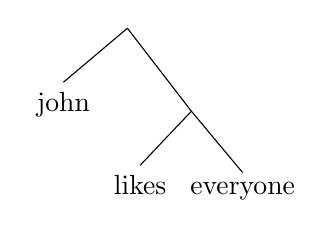
\begin{tikzpicture}
      \Tree [ john [ likes everyone ] ]
    \end{tikzpicture}
  \end{minipage}%
  \begin{minipage}{0.02\linewidth}
    $\equiv$
  \end{minipage}%
  \begin{minipage}{0.4\linewidth}
    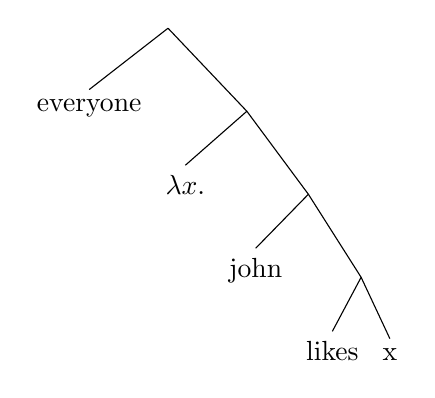
\begin{tikzpicture}
      \Tree [ everyone [ $\lambda x.$ [ john [ likes x ] ] ] ]
    \end{tikzpicture}
  \end{minipage}
\end{center}
To achieve this, they add a new mode to NL---that is to say, a copy of
the rules for $\{\impr,\prod,\impl\}$ applying to three new connectives
$\{\himpr,\hprod,\himpl\}$---and the following (somewhat controversial)
equivalence on structures:
\[
  \Sigma[\Delta]\equiv\Delta\circ\lambda x.\Sigma[x]
\]
This equivalence is intuitive, and works as expected. For instance,
using display NL extended with this equivalence, we can easily give a
derivation for ``John likes everyone,'' using the type
$\S\himpl(\NP\himpr\S)$ for quantifiers:
\begin{pfblock}
  \AXC{$\vdots$}\noLine
  \UIC{$\struct{\NP}\prod\struct{(\NP\impr\S)\impl\NP}\prod\struct{\NP}
    \fCenter\struct{\S}$}
  \RightLabel{$\lambda$}
  \UIC{$\struct{\NP}\hprod\lambda{x}.
    (\struct{\NP}\prod\struct{(\NP\impr\S)\impl\NP}\prod x)\fCenter\struct{\S}$}
  \RightLabel{Res$\hprod\himpr$}
  \UIC{$\lambda{x}.(\struct{\NP}\prod\struct{(\NP\impr\S)\impl\NP}\prod{x})
    \fCenter\struct{\NP}\himpr\struct{\S}$}
  \RightLabel{R$\himpr$}
  \UIC{$\lambda{x}.(\struct{\NP}\prod\struct{(\NP\impr\S)\impl\NP}\prod{x})
    \fCenter\struct{\NP\himpr\S}$}
  \AXC{}\RightLabel{Ax}\UIC{$\struct{S}\fCenter\struct{S}$}
  \BIC{$\struct{\S\himpl(\NP\himpr\S)}\fCenter\struct{\S}\himpl\lambda{x}.
    (\struct{\NP}\prod\struct{(\NP\impr\S)\impl\NP}\prod x)$}
  \RightLabel{Res$\himpl\:\hprod$}
  \UIC{$\struct{\S\himpl(\NP\himpr\S)}\hprod\lambda{x}.
    (\struct{\NP}\prod\struct{(\NP\impr\S)\impl\NP}\prod x)\fCenter\struct{\S}$}
  \RightLabel{$\lambda$}
  \UIC{$\struct{\NP}\prod\struct{(\NP\impr\S)\impl\NP}\prod\struct{\S\himpl
      (\NP\himpr\S)}\fCenter\struct{\S}$}
\end{pfblock}
However, the use of a binding construct in the syntax for structures
makes this equivalence quite difficult to formalise.
In addition, if we were to take the equivalence at face value, we
would end up with a logic in which we could do all kinds of unpleasant
things. For instance, since contexts are defined as structures with a
hole, we could raise quantifiers past one another, indefinitely:
\begin{pfblock}
  \AXC{$\vdots$}\noLine
  \UIC{$\struct{{\S\impl(\NP\impr\S)}}\hprod\lambda{z}.(\struct{{\S\impl(\NP\impr\S)}}\hprod\lambda{y}.({z}\hprod\lambda{x}.({y}\prod\struct{(\NP\impr\S)\impl\NP}\prod{x})))\fCenter\struct{\S}$}
  \RightLabel{$\lambda$}
  \UIC{$\struct{{\S\impl(\NP\impr\S)}}\hprod\lambda{y}.(\struct{{\S\impl(\NP\impr\S)}}\hprod\lambda{x}.({y}\prod\struct{(\NP\impr\S)\impl\NP}\prod{x}))\fCenter\struct{\S}$}
  \RightLabel{$\lambda$}
  \UIC{$\struct{{\S\impl(\NP\impr\S)}}\hprod\lambda{x}.(\struct{{\S\impl(\NP\impr\S)}}\prod\struct{(\NP\impr\S)\impl\NP}\prod{x})\fCenter\struct{\S}$}
  \RightLabel{$\lambda$}
  \UIC{$\struct{{\S\impl(\NP\impr\S)}}\prod\struct{(\NP\impr\S)\impl\NP}\prod\struct{{\S\impl(\NP\impr\S)}}\fCenter\struct{\S}$}
\end{pfblock}
Or, as \citet{barker2015} note, we could lift variables out of the
scope of their binder:
\begin{pfblock}
  \AXC{$\vdots$}\noLine
  \UIC{${x}\hprod\lambda{y}.(\struct{{\S\impl(\NP\impr\S)}}\hprod\lambda{x}.(\struct{{\S\impl(\NP\impr\S)}}\prod\struct{(\NP\impr\S)\impl\NP}\prod{y}))\fCenter\struct{\S}$}
  \RightLabel{$\lambda$}
  \UIC{$\struct{{\S\impl(\NP\impr\S)}}\hprod\lambda{x}.(\struct{{\S\impl(\NP\impr\S)}}\prod\struct{(\NP\impr\S)\impl\NP}\prod{x})\fCenter\struct{\S}$}
  \RightLabel{$\lambda$}
  \UIC{$\struct{{\S\impl(\NP\impr\S)}}\prod\struct{(\NP\impr\S)\impl\NP}\prod\struct{{\S\impl(\NP\impr\S)}}\fCenter\struct{\S}$}
\end{pfblock}
Needless to say, any logic extended with this equivalence loses a
number of pleasant properties, one of which is decidable proof
search. However, in chapter 17 of their book, \citeauthor{barker2015}
do a great job of capturing the essence of the $\lambda$-rule in a
logical manner; while their system is not yet decidable, it is very
nearly so. They extend NL by a second modality
$\{\himpr,\hprod,\himpl\}$, add three primitive structural constants
$\{\I,\B,\C\}$, and add the following structural rules:
\begin{center}
  \begin{pfbox}
    \AXC{$X\fCenter Y$}
    \doubleLine\RightLabel{\I}
    \UIC{$X\hprod\I\fCenter Y$}
  \end{pfbox}
  \begin{pfbox}
    \AXC{$X\prod(Y\hprod Z)\fCenter W$}
    \doubleLine\RightLabel{\B}
    \UIC{$Y\hprod((\B\prod X)\prod Z)\fCenter W$}
  \end{pfbox}
  \begin{pfbox}
    \AXC{$(X\prod Y)\hprod Z\fCenter W$}
    \doubleLine\RightLabel{\C}
    \UIC{$X\hprod((\C\prod Y)\prod Z)\fCenter W$}
  \end{pfbox}
\end{center}
They call the result NL$_{\text{CL}}$ (and, occasionally,
NL$_{\text{IBC}}$). In this calculus, quantifier raising can be done
in much the same way as in NL$_\lambda$---though the new version is
ever so slightly more verbose:\footnote{%
  Inverted applications of the \I, \B\ and \C\ rules are marked with a prime.
}
\begin{pfblock}
  \AXC{$\vdots$}\noLine
  \UIC{$\struct{\NP}\prod\struct{(\NP\impr\S)\impl\NP}\prod\struct{{\NP}}\fCenter\struct{{\S}}$}
  \RightLabel{Res$\prod\impr$}
  \UIC{$\struct{(\NP\impr\S)\impl\NP}\prod\struct{{\NP}}\fCenter\struct{\NP}\impr\struct{{\S}}$}
  \RightLabel{Res$\prod\impr$}
  \UIC{$\struct{{\NP}}\fCenter\struct{(\NP\impr\S)\impl\NP}\impr\struct{\NP}\impr\struct{{\S}}$}
  \RightLabel{\I}
  \UIC{$\struct{{\NP}}\hprod\I\fCenter\struct{(\NP\impr\S)\impl\NP}\impr\struct{\NP}\impr\struct{{\S}}$}
  \RightLabel{Res$\impr\prod$}
  \UIC{$\struct{(\NP\impr\S)\impl\NP}\prod(\struct{{\NP}}\hprod\I)\fCenter\struct{\NP}\impr\struct{{\S}}$}
  \RightLabel{\B}
  \UIC{$\struct{{\NP}}\prod((\B\prod\struct{(\NP\impr\S)\impl\NP})\prod\I)\fCenter\struct{\NP}\impr\struct{{\S}}$}
  \RightLabel{Res$\prod\impr$}
  \UIC{$\struct{\NP}\prod(\struct{{\NP}}\hprod((\B\prod\struct{(\NP\impr\S)\impl\NP})\prod\I))\fCenter\struct{{\S}}$}
  \RightLabel{\B}
  \UIC{$\struct{{\NP}}\hprod((\B\prod\struct{\NP})\prod((\B\prod\struct{(\NP\impr\S)\impl\NP})\prod\I))\fCenter\struct{{\S}}$}
  \RightLabel{Res$\hprod\himpr$}
  \UIC{$((\B\prod\struct{\NP})\prod((\B\prod\struct{(\NP\impr\S)\impl\NP})\prod\I))\fCenter\struct{{\NP}}\himpr\struct{{\S}}$}
  \RightLabel{R$\himpr$}
  \UIC{$((\B\prod\struct{\NP})\prod((\B\prod\struct{(\NP\impr\S)\impl\NP})\prod\I))\fCenter\struct{{\NP\himpr\S}}$}
  \AXC{}\RightLabel{Ax}\UIC{$\struct{\S}\fCenter\struct{{\S}}$}
  \RightLabel{L$\himpl$}
  \BIC{$\struct{{\S\himpl(\NP\himpr\S)}}\fCenter\struct{\S}\himpl((\B\prod\struct{\NP})\prod((\B\prod\struct{(\NP\impr\S)\impl\NP})\prod\I))$}
  \RightLabel{Res$\himpl\:\hprod$}
  \UIC{$\struct{{\S\himpl(\NP\himpr\S)}}\hprod((\B\prod\struct{\NP})\prod((\B\prod\struct{(\NP\impr\S)\impl\NP})\prod\I))\fCenter\struct{\S}$}
  \RightLabel{$\B'$}
  \UIC{$\struct{\NP}\prod(\struct{{\S\himpl(\NP\himpr\S)}}\hprod((\B\prod\struct{(\NP\impr\S)\impl\NP})\prod\I))\fCenter\struct{\S}$}
  \RightLabel{Res$\prod\impr$}
  \UIC{$\struct{{\S\himpl(\NP\himpr\S)}}\hprod((\B\prod\struct{(\NP\impr\S)\impl\NP})\prod\I)\fCenter\struct{\NP}\impr\struct{\S}$}
  \RightLabel{$\B'$}
  \UIC{$\struct{(\NP\impr\S)\impl\NP}\prod(\struct{{\S\himpl(\NP\himpr\S)}}\hprod\I)\fCenter\struct{\NP}\impr\struct{\S}$}
  \RightLabel{Res$\impr\prod$}
  \UIC{$\struct{{\S\himpl(\NP\himpr\S)}}\hprod\I\fCenter\struct{(\NP\impr\S)\impl\NP}\impr\struct{\NP}\impr\struct{\S}$}
  \RightLabel{$\I'$}
  \UIC{$\struct{{\S\himpl(\NP\himpr\S)}}\fCenter\struct{(\NP\impr\S)\impl\NP}\impr\struct{\NP}\impr\struct{\S}$}
  \RightLabel{Res$\prod\impr$}
  \UIC{$\struct{(\NP\impr\S)\impl\NP}\prod\struct{{\S\himpl(\NP\himpr\S)}}\fCenter\struct{\NP}\impr\struct{\S}$}
  \RightLabel{Res$\prod\impr$}
  \UIC{$\struct{\NP}\prod\struct{(\NP\impr\S)\impl\NP}\prod\struct{{\S\himpl(\NP\himpr\S)}}\fCenter\struct{\S}$}
\end{pfblock}
One of the advantages of this formalisation is that it gets rid of the
awkward binding construct in the syntax of structures. In addition, it
makes it clear that quantifiers can only move past \emph{solid}
products. However, it is not entirely free of problems. One of the
more glaring problems is that using this encoding, any expression can
be the subject of quantifier raising. For instance, in ``John likes
Mary,'' we could choose to raise the verb:
\begin{pfblock}
  \AXC{$\vdots$}\noLine
  \UIC{$\struct{{(\NP\impr\S)\impl\NP}}\hprod(\B\prod\struct{\NP})
    \prod((\C\prod\I)\prod\struct{\NP})\fCenter\struct{\S}$}\noLine
  \UIC{$\vdots$}\noLine
  \UIC{$\struct{\NP}\prod\struct{{(\NP\impr\S)\impl\NP}}\prod\struct{\NP}\fCenter\struct{\S}$}
\end{pfblock}
Since verbs are usually not considered scope-takers, it is unlikely
that raising the verb would lead to anything other then lowering it
again. However, the fact that we leave it open as an opportunity is
wasted computational effort; while all futile attempts at raising and
lowering will lead to a loop, and therefore spare us the spurious
ambiguity, there are still a great deal of futile attempts to be made.

Another problem is the $\I'$-rule. It allows us to introduce an
arbitrary amount of \I's, which causes a \emph{growing} loop in our
proof search procedure:
\begin{pfblock}
  \AXC{$\vdots$}\noLine
  \UIC{$((\struct{\NP}\prod\struct{\NP\impr\S})\hprod\I)\hprod\I\fCenter\struct{\S}$}
  \RightLabel{$\I'$}
  \UIC{$(\struct{\NP}\prod\struct{\NP\impr\S})\hprod\I\fCenter\struct{\S}$}
  \RightLabel{$\I'$}
  \UIC{$\struct{\NP}\prod\struct{\NP\impr\S}\fCenter\struct{\S}$}
\end{pfblock}
I propose to handle both of these issues with one simple addition. The
idea is to add a new unary connective, $\q[A]$, which represents a
license to perform quantifier raising. Since we want to replace the
problematic $\I'$-rule, we will choose the structural version of our
quantifying license to be a \emph{hollow} product with a right-hand
unit. On the other side, since we do not want logical products, we
will keep $\q[A]$ it as an atomic logical connective. This gives us
the following logical left rule:
\begin{pfblock}
  \AXC{$\struct{A}\hprod\I\fCenter Δ$}
  \RightLabel{L\I}
  \UIC{$\struct{\q[A]}\fCenter Δ$}
\end{pfblock}
The appropriate right rule is easily derived from the conventional
display calculus rules for products and units---though I do not imagine
we will generally want to see quantifying licenses in our output type:
\begin{pfblock}
  \AXC{$Γ\fCenter\struct{B}$}
  \RightLabel{R\I}
  \UIC{$Γ\hprod\I\fCenter\struct{\q[B]}$}
\end{pfblock}
And indeed, the pair obeys all constraints imposed by display
calculus, including a valid proof for \textbf{C8}:
\begin{pfblock}
  \AXC{$Γ\fCenter\struct{A}$}
  \AXC{$\struct{A}\hprod\I\fCenter Δ$}
  \RightLabel{Res$\hprod\himpl$}
  \UIC{$\struct{A}\fCenter Δ\himpl\I$}
  \RightLabel{Cut}
  \BIC{$Γ\fCenter Δ\himpl\I$}
  \RightLabel{Res$\himpl\hprod$}
  \UIC{$Γ\hprod\I\fCenter Δ$}
\end{pfblock}
Note that we keep the $\I$-rule, though we rename it $\I^-$ to
emphasise that it can now only \emph{remove} $\I$s. The full
extension, including semantics, and focused rules, can be found in
\autoref{fig:extension-quantifier-raising}. The semantics are rather
trivial: we simply translate all constants as units, and translate
$\q[A]$ as $A$, inserting and removing the right unit as needed.

\begin{figure}[hb]
  \begin{mdframed}
    \centering
    \begin{minipage}{0.666\linewidth}
      \centering
      \begin{alignat*}{4}
        \text{Type}     &  \;&A,B&\coloneqq\ldots\vsep A\himpr B\vsep B\himpl A\vsep\q[A]\\
        \text{Structure}&^+\;&Γ  &\coloneqq\ldots\vsep Γ_1\hprod Γ_2\vsep\I\vsep\B\vsep\C\\
        \text{Structure}&^-\;&Δ  &\coloneqq\ldots\vsep Γ\himpr Δ\vsep Δ\himpl Γ
      \end{alignat*}
    \end{minipage}%
    \begin{minipage}{0.333\linewidth}
      \centering
      \begin{alignat*}{4}
        &\text{Pol}(A\himpr B) &&\mapsto{-}\\
        &\text{Pol}(B\himpl A) &&\mapsto{-}\\
        &\text{Pol}(\q[A])    &&\mapsto{+}
      \end{alignat*}
    \end{minipage}
    \\[1\baselineskip]
    (copy of rules for $\{\impr,\prod,\impl\}$ from
    \autoref{fig:display-calculus} for $\{\himpr,\hprod,\himpl\}$)
    \\[1\baselineskip]
    \begin{pfbox}
      \AXC{$\struct{A}\hprod\I\fCenter Δ$}
      \RightLabel{L\I}
      \UIC{$\struct{\q[A]}\fCenter Δ$}
    \end{pfbox}
    \begin{pfbox}
      \AXC{$Γ\fCenter\focus{B}$}
      \RightLabel{R\I}
      \UIC{$Γ\hprod\I\fCenter\focus{\q[B]}$}
    \end{pfbox}
    \begin{pfbox}
      \AXC{$Γ\fCenter Δ$}
      \RightLabel{$\I^-$}
      \UIC{$Γ\hprod\I\fCenter Δ$}
    \end{pfbox}
    \\[1\baselineskip]
    \begin{pfbox}
      \AXC{$Γ_1\prod(Γ_2\hprod Γ_3)\fCenter Δ$}
      \doubleLine\RightLabel{\B}
      \UIC{$Γ_2\hprod((\B\prod Γ_1)\prod Γ_3)\fCenter Δ$}
    \end{pfbox}
    \begin{pfbox}
      \AXC{$(Γ_1\hprod Γ_2)\prod Γ_3\fCenter Δ$}
      \doubleLine\RightLabel{\C}
      \UIC{$Γ_1\hprod((\C\prod Γ_2)\prod Γ_3)\fCenter Δ$}
    \end{pfbox}
    \\[1\baselineskip]
    \hrulefill
    \\[1\baselineskip]
    {
      \renewcommand{\arraystretch}{1.5}%
      \(\!
      \begin{array}{c c c}
        \multicolumn{3}{c}{\tr[({\q[A]})]\mapsto\tr[A]}\\
        \tr[\I]\mapsto\top      & \tr [\B]\mapsto\top     & \tr [\C]\mapsto\top\\
      \end{array}
      \)
    }
    \\[1\baselineskip]
    (copy of translations for $\{\impr,\prod,\impl\}$ from
    \autoref{fig:display-calculus-to-explicit-lamET} for
    $\{\himpr,\hprod,\himpl\}$)
    \\[1\baselineskip]
    \begin{pfbox}
      \AXC{$x:\struct{A}\hprod\I\fCenter M:Δ$}
      \RightLabel{L\I}
      \UIC{$y:\struct{\q[A]}\fCenter \sub{M}{(y,())}{x}:Δ$}
    \end{pfbox}
    \begin{pfbox}
      \AXC{$x:Γ\fCenter\focus{M:B}$}
      \RightLabel{R\I}
      \UIC{$y:Γ\hprod\I\fCenter\focus{\sub{M}{\fst{y}}{x}:\q[B]}$}
    \end{pfbox}
    \begin{pfbox}
      \AXC{$x:Γ\fCenter M:Δ$}
      \RightLabel{$\I^-$}
      \UIC{$y:Γ\hprod\I\fCenter \sub{M}{\fst{y}}{x}:Δ$}
    \end{pfbox}
    \\[1\baselineskip]
    (where $\fst{x}=\case{x}{y}{z}{y}$)
    \\[1\baselineskip]
    (\B\ and \C\ translate to various combinations of associativity,
    commutativity, $\emptyset$E and weakening)
    \\
    \vspace*{\baselineskip}
  \end{mdframed}
  \caption{
    Extension of calculus in \autoref{fig:display-calculus} which
    supports quantifier raising.}%
  \label{fig:extension-quantifier-raising}
\end{figure}

%%% Local Variables:
%%% mode: latex
%%% TeX-master: t
%%% End:


The extension presented so far for quantifier raising is pretty good:
because we have removed all growing loops in structural rules, it now
has a decidable and complete procedure for proof search, and it neatly
captures quantifier movement---i.e. moving upwards, taking scope,
binding a variable, and moving that variable back down. However, it
still has one problem: spurious ambiguity. Imagine a sentence with two
quantifiers $P$ and $Q$, respectively \emph{one} and \emph{two} places
removed from the top of the syntax tree. The ambiguity that we want is
``do we raise $P$ first, or do we raise $Q$ first?'' However, in
addition to these possibilities, we now also have to possibility to
raise $Q$ one step, then raise $P$, and then raise $Q$ a second
step---semantically, this is equivalent to raising $P$, then
$Q$. NL$_\lambda$---if you only allow quantifier raising past solid
products---does not have this problem.

\citet[][chapter 17.6]{barker2015} examine the restrictions that need
to be put on the $\lambda$-rule in order to be able to translate
NL$_\lambda$ to NL$_{\text{CL}}$. In order to keep our structural
rules simple, and our calculus free of structural lambdas, I opt to go
the other way around, and see how close we can get to defining the
$\lambda$-rule in our calculus in \autoref{fig:extension-quantifier-raising}.
For this, we will need the following definitions:
\begin{center}
  $\text{Context}\;Σ\coloneqq\Box\vsep Σ\prodl Γ\vsep Γ\prodr Σ$\\
  \begin{minipage}{0.45\linewidth}
    \begin{alignat*}{2}
      &\Box       \;&&[Γ']\mapsto Γ'\\
      &(Σ\prodl Γ)\;&&[Γ']\mapsto (Σ[Γ']\prod Γ)\\
      &(Γ\prodr Σ)\;&&[Γ']\mapsto (Γ\prod Σ[Γ'])
    \end{alignat*}
  \end{minipage}
  \begin{minipage}{0.45\linewidth}
    \begin{alignat*}{2}
      &\trace(\Box)     \;&&\mapsto \mathbf{I}\\
      &\trace(Σ\prodl Γ)\;&&\mapsto ((\mathbf{C}\prod \trace(Σ))\prod Γ)\\
      &\trace(Γ\prodr Σ)\;&&\mapsto ((\mathbf{B}\prod Γ)\prod
      \trace(Σ))
    \end{alignat*}
  \end{minipage}
\end{center}
First we have contexts, which encode structures with a single hole,
where the nodes leading up to the hole are all solid
products---exactly the type of structure that quantifiers can move up
through. The syntax is a little abusive, as we use the same symbol for
products, products with a hole in their left argument, and products
with a hole in their right argument. However, as we require that
contexts have only a single hole, it is always unambiguous. Note that
products are right-associative.
Secondly, we have the plugging function `$\plug$', which inserts some
structure into the single hole in a context.
Lastly, the `trace' function computes, from a context, the trace of
$\B$s and $\C$s that would be left after something quantifies out of
that context.

Given these definitions, we can show that the following rule for
quantifier movement is admissible, by induction on the structure of
the context:
\begin{pfblock}
  \AXC{$\struct{A}\hprod\trace(Σ)\fCenter Δ$}
  \doubleLine\RightLabel{$\uparrow\downarrow$}
  \UIC{$Σ[\struct{\q[A]}]\fCenter Δ$}
\end{pfblock}
This new rule is very close to \citeauthor{barker2015}'s equivalence,
with as its only difference that the quantifying license is now built
into it:
\[
  \Sigma[\Delta]\equiv\Delta\circ\lambda x.\Sigma[x]
  \qquad
  Σ[\struct{\q[A]}]\equiv\struct{A}\hprod\trace(Σ)
\]
In fact, if you read products as function applications, and the
constants $\{\I,\B,\C\}$ as the combinators, as \citet{barker2015}
intended, then the right-hand side expressions are more-or-less
equivalent.\footnote{%
  As an aside: what we set out to encode were contexts with holes that
  are unique---plugging should never duplicate or forget
  information. So the $\lambda$-terms in NL$_\lambda$ were implicitly
  linear. The combinators $\I$, $\B$ and $\C$ correspond precisely to
  the linear lambda calculus. However, the combinator language is far
  easier to encode than linear binding constructs.
}
Proof search with this derived rule is still complete; it merely
enforces that the entire quantifier raising or lowering is done in one
go.\todo{No proof.}

In their discussion of decidability, \citet{barker2015} derive the
`expansion' and `reduction' rules which more-or-less correspond to
the two directions of the equivalence, or the two directions of our
$\uparrow\downarrow$-rule. They then combine these rules with
L$\himpl$ and R$\himpr$, respectively, yielding the
$\himpl\,\text{L}_\lambda$ and $\himpr\text{R}_\lambda$ rules. The
advantage of these combined rules is that they obey the sub-formula
property, and are therefore suited to naive backward-chaining proof
search. We can do a similar thing using our $\uparrow\downarrow$-rule:
\begin{center}
  \begin{pfbox}
    \AXC{$\trace(Σ)\fCenter\struct{A\himpr B}$} \AXC{$\struct{C}\fCenter Δ$}
    \RightLabel{\qup}
    \BIC{$Σ[\struct{\q[C\himpl(A\himpr B)]}]\fCenter Δ$}
  \end{pfbox}
  \begin{pfbox}
    \AXC{$Σ[\struct{A}]\fCenter\struct{B}$}
    \RightLabel{\qdown}
    \UIC{$\trace(Σ)\fCenter\struct{A\himpr B}$}
  \end{pfbox}
\end{center}
While proof search with these rules is decidable, it is no longer
complete. However, it \emph{is} complete for the fragment of display
NL where all types involving a quantifying license are of the form
$\q[C\himpl(A\himpr B)]$, which is what we can reasonably expect from
natural language.
In addition, proof search using these rules is no longer plagued by
the spurious ambiguity that resulted from the $\B$ and $\C$
rules---and, to boot, we can write proofs involving quantifier
movement in a much more succinct manner:
\begin{pfblock}
  \AXC{$\vdots$}\noLine
  \UIC{$\struct{\NP}\prod\textsc{loves}\prod\struct{\NP}\fCenter\struct{\S}$}
  \RightLabel{\qdown}
  \UIC{$\trace(\Box\prod\textsc{loves}\prod\struct{\NP})\fCenter\struct{{\NP\himpr\S}}$}
  \AXC{}\RightLabel{Ax}\UIC{$\struct{\S}\fCenter\struct{\S}$}
  \RightLabel{\qup}
  \BIC{$\textsc{everyone}\prod\textsc{loves}\prod\struct{\NP}\fCenter\struct{\S}$}
  \RightLabel{\qdown}
  \UIC{$\trace(\textsc{everyone}\prod\textsc{loves}\prod\Box)\fCenter\struct{{\NP\himpr\S}}$}
  \AXC{}\RightLabel{Ax}\UIC{$\struct{\S}\fCenter\struct{\S}$}
  \RightLabel{\qup}
  \BIC{$\textsc{everyone}\prod\textsc{loves}\prod\textsc{someone}\fCenter\struct{\S}$}
\end{pfblock}
\vspace*{-1\baselineskip}
\begin{gather*}
  \downmapsto
  \\
  (\someone\;(\lambda y. \everyone\;(\lambda x.\likes\;y\;x)))
  \\
  \downmapsto
  \\
  \exists y.\PERSON(y)\wedge\forall x.\PERSON(x)\supset\LIKE(x,y)
\end{gather*}
Note that though we have the option, we do not have to unfold the
application of `trace' in this particular proof. In future proofs, if
we choose to fold or unfold an application of `trace', we will
explicitly mark this as an application of rewriting by equality
(`$=$').

\begin{landscape}
  \begin{figure}
    \begin{mdframed}
      \centering
      \begin{pfblock}[0.74]
        \AXC{$\vdots$}\noLine
        \UIC{$
          \textsc{the}\prod\textsc{author}\prod\textsc{of}\prod\struct\NP
          \fCenter\struct\NP$}
        \RightLabel{\qdown}
        \UIC{$
          \trace(\textsc{the}\prod\textsc{author}\prod\textsc{of}\prod\Box)
          \fCenter\struct{\NP\himpl\NP}$}
        \AXC{$\vdots$}\noLine
        \UIC{$
          \NP\prod\textsc{feared}\prod\textsc{the}\prod\textsc{ocean}\fCenter\struct{\S}$}
        \RightLabel{DP}
        \UIC{$
          \textsc{feared}\prod\textsc{the}\prod\textsc{ocean}\fCenter\struct{\NP\impr\S}$}
        \AXC{$\vdots$}\noLine
        \UIC{$\struct{\N\impr\N}\fCenter\textsc{book}\impr\struct\N$}
        \RightLabel{L$\impl$}
        \BIC{$
          \struct{(\N\impr\N)\impl(\NP\impr\S)}
          \fCenter(\textsc{book}\impr\struct\N)\impl
          (\textsc{feared}\prod\textsc{the}\prod\textsc{ocean})$}
        \RightLabel{\qup}
        \BIC{$
          \textsc{the}\prod\textsc{author}\prod\textsc{of}\prod\textsc{which}
          \fCenter(\textsc{book}\impr\struct\N)\impl(\textsc{feared}\prod
          \textsc{the}\prod\textsc{ocean})$}
        \RightLabel{DP}
        \UIC{$
          \textsc{book}\prod(\textsc{the}\prod\textsc{author}\prod\textsc{of}\prod
          \textsc{which})\prod\textsc{feared}\prod\textsc{the}\prod\textsc{ocean}
          \fCenter\struct\N$}
        \AXC{$\vdots$}\noLine
        \UIC{$
          \textsc{alice}\prod\textsc{read}\prod\struct\NP
          \fCenter\struct\S$}
        \RightLabel{\qdown}
        \UIC{$
          \trace(\textsc{alice}\prod\textsc{read}\prod\Box)
          \fCenter\struct{\S\himpl\NP}$}
        \AXC{}\RightLabel{Ax}\UIC{$\struct\S\fCenter\struct\S$}
        \RightLabel{\qup}
        \BIC{$
          \textsc{alice}\prod\textsc{read}\prod\q[(\S\himpl\NP)\himpr\S]
          \fCenter\struct{\S}$}
        \RightLabel{DP}
        \UIC{$
          \q[(\S\himpl\NP)\himpr\S]
          \fCenter\textsc{read}\impr(\textsc{alice}\impr\struct{\S})$}
        \RightLabel{L$\impl$}
        \BIC{$
          \textsc{a}\fCenter(\textsc{read}\impr(\textsc{alice}\impr\struct{\S}))\impl
          (\textsc{book}\prod(\textsc{the}\prod\textsc{author}\prod\textsc{of}\prod
          \textsc{which})\prod\textsc{feared}\prod\textsc{the}\prod\textsc{ocean})$}
        \RightLabel{DP}
        \UIC{$
          \textsc{alice}\prod\textsc{read}\prod\textsc{a}\prod\textsc{book}\prod
          (\textsc{the}\prod\textsc{author}\prod\textsc{of}\prod\textsc{which})\prod
          \textsc{feared}\prod\textsc{the}\prod\textsc{ocean}\fCenter\struct{\S}$}
      \end{pfblock}
      \vspace*{-1\baselineskip}
      \begin{gather*}
        \downmapsto
        \\
        \text{a}\;(\lambda{x}.\text{which}\;
          (\lambda{z}.\text{the}\;(\text{of}\;z\;\text{author}))\;
          (\lambda{w}.\text{fear}\;(\text{the}\;\text{ocean})\;w)\;
          \text{book}\;x)\;
          (\lambda{y}.\text{read}\;y\;\text{alice})
        \\
        \downmapsto
        \\
        \exists{x}.
        (\BOOK(x)\wedge\PAST(\FEAR(\iota(\lambda{y}.\OF(y,\AUTHOR,x)),\iota(\OCEAN)))
        \wedge\PAST(\READ(\ALICE,x))
      \end{gather*}
    \end{mdframed}
    \caption{An example of changing answer types.}
    \label{fig:example-changing-answer-type}
  \end{figure}
\end{landscape}
%
%%% Local Variables:
%%% mode: latex
%%% TeX-master: t
%%% End:


\paragraph{Parasitic scope}
The system described in \autoref{fig:extension-quantifier-raising}
maintains the decomposition of the quantifier movement into two
separate functions---raising and lowering. Therefore, we can still
analyse parasitic scope \citep{barker2007}. In
\autoref{fig:parasitic-scope}, we analyse a classic example of
parasitic scope for \emph{different}: ``A different waiter served
everyone.'' However, we make one small change to the type of
`different', in order to obtain the semantics described by
\citet{kiselyov2015b}. We use the lexicon described below:
\[
  \renewcommand*{\arraystretch}{1}
  \begin{array}{l c l}
    \multirow{2}{*}{\a}
    &:& \tr[{(\q[\S\himpl(\NP\himpr\S)]\impl\N)}]\\
    &=& \lambda n. \lambda k. \exists x. n\;x\wedge k\;x\\

    \multirow{2}{*}{\different}
    &:& \tr[{(\q[\S\himpl(\q[(\NP\himpr\S)\himpl(\A\himpr(\NP\himpr\S))]\himpr\S)])}]\\
    &=& \lambda k. \exists f. (\forall x.\forall y.\nexists z.f\;z\;x\wedge f\;z\;y)\;\wedge\\
    & & k\;(\lambda k'.\lambda x.k'\;(\lambda g.\lambda y.g\;y\wedge f\;x\;y)\;x)\\

    \multirow{2}{*}{\waiter}
    &:& \tr[\N]\\
    &=& \lambda x.\WAITER(x)\\

    \multirow{2}{*}{\served}
    &:& \tr[\TV]\\
    &=& \lambda y.\lambda x.\PAST(\SERVE(x,y))\\

    \multirow{2}{*}{\everyone}
    &:& \tr[{(\q[\S\himpl(\NP\himpr\S)])}]\\
    &=& \lambda k.\forall x.\PERSON(x)\supset k\;x
  \end{array}
\]
It may be worthwhile to have a closer look at the type for
`different.' It is a quantifier taking scope at the sentence
level ${\q[\S\himpl(\ldots\himpr\S)]}$, which becomes a quantifier
taking scope parasitically ${\q[(\NP\himpr\S)\himpl(\ldots
\himpr(\NP\himpr\S))]}$, and finally becomes an adjective $\A$.

The double quantification in `different' has some very interesting
effects. Because it takes scope normally and then parasitically the
sentence ``A different waiter served everyone'' is unambiguous, even
though it contains no fewer than \emph{three} quantifiers. This is
because of the dependencies between the quantifiers: `a' cannot take
scope until it receives its noun argument, which is modified by
`different'. Meanwhile, `different' has to take scope twice, once
normally and once parasitically. Its parasitic scope-taking has to
occur \emph{while} `everyone' is taking scope, so its normal
scope-taking has to occur before that.
On the semantic level, double quantification allows a quantifier to
capture another quantifier while \emph{also} taking scope over it.

\begin{landscape}
  \begin{figure}
    \begin{mdframed}
      \vspace*{0.5\baselineskip}
      \begin{pfblock}[0.85]
        \AXC{}\RightLabel{Ax}\UIC{$\textsc{waiter}\fCenter\struct{\N}$}
        \AXC{}\RightLabel{Ax}\UIC{$\struct{\N}\fCenter\struct{\N}$}
        \AXC{$\vdots$}\noLine
        \UIC{$\struct{\NP}\prod\textsc{served}\prod\struct{\NP}\fCenter\struct{\S}$}
        \RightLabel{\qdown}
        \UIC{$\trace(\Box\prodl\textsc{served}\prod\struct{\NP})\fCenter\struct{\NP\himpr\S}$}
        \AXC{}\RightLabel{Ax}\UIC{$\struct{\S}\fCenter\struct{\S}$}
        \RightLabel{\qup}
        \BIC{$\struct{\q[\S\himpl(\NP\himpr\S)]}\prod\textsc{served}\prod\struct{\NP}\fCenter\struct{\S}$}
        \RightLabel{Res$\prod\impl$}
        \UIC{$\struct{\q[\S\himpl(\NP\himpr\S)]}\fCenter\struct{\S}\impl(\textsc{served}\prod\struct{\NP})$}
        \RightLabel{L$\impl$}
        \BIC{$\textsc{a}\fCenter(\struct{\S}\impl(\textsc{served}\prod\struct{\NP}))\impl\struct{\N}$}
        \RightLabel{Res$\impl\prod$}
        \UIC{$\textsc{a}\prod\struct{\N}\fCenter\struct{\S}\impl(\textsc{served}\prod\struct{\NP})$}
        \RightLabel{Res$\prod\impr$}
        \UIC{$\struct{\N}\fCenter\textsc{a}\impr(\struct{\S}\impl(\textsc{served}\prod\struct{\NP}))$}
        \RightLabel{L$\impl$}
        \BIC{$\struct{\A}\fCenter(\textsc{a}\impr(\struct{\S}\impl(\textsc{served}\prod\struct{\NP})))\impl\textsc{waiter}$}
        \RightLabel{Res$\impl\prod$}
        \UIC{$\struct{\A}\prod\textsc{waiter}\fCenter\textsc{a}\impr(\struct{\S}\impl(\textsc{served}\prod\struct{\NP}))$}
        \RightLabel{Res$\impr\prod$}
        \UIC{$\textsc{a}\prod\struct{\A}\prod\textsc{waiter}\fCenter\struct{\S}\impl(\textsc{served}\prod\struct{\NP})$}
        \RightLabel{Res$\impl\prod$}
        \UIC{$(\textsc{a}\prod\struct{\A}\prod\textsc{waiter})\prod\textsc{served}\prod\struct{\NP}\fCenter\struct{\S}$}
        \RightLabel{\qdown}
        \UIC{$\trace((\textsc{a}\prod\struct{\A}\prod\textsc{waiter})\prodr\textsc{served}\prodr\Box)\fCenter\struct{\NP\himpr\S}$}
        \RightLabel{$=$}
        \UIC{$(\B\prod\textsc{a}\prod\struct{\A}\prod\textsc{waiter})\prod(\B\prod\textsc{served})\prod\I)\fCenter\struct{\NP\himpr\S}$}
        \RightLabel{\qdown}
        \UIC{$\trace((\B\prodr\textsc{a}\prodr\Box\prodl\textsc{waiter})\prodl(\B\prod\textsc{served})\prod\I)\fCenter\struct{\A\himpr(\NP\himpr\S)}$}
        \AXC{}\RightLabel{Ax}\UIC{$\struct{\S}\fCenter\struct{\S}$}
        \RightLabel{\qup}
        \BIC{$(\B\prod\textsc{a}\prod\q[(\NP\himpr\S)\himpl(\A\himpr(\NP\himpr\S))]\prod\textsc{waiter})\prod(\B\prod\textsc{served})\prod\I\fCenter\struct{\NP\himpr\S}$}
        \RightLabel{$=$}
        \UIC{$\trace((\textsc{a}\prod\q[(\NP\himpr\S)\himpl(\A\himpr(\NP\himpr\S))]\prod\textsc{waiter})\prodr\textsc{served}\prodr\Box)\fCenter\struct{\NP\himpr\S}$}
        \AXC{}\RightLabel{Ax}\UIC{$\struct{\S}\fCenter\struct{\S}$}
        \RightLabel{\qup}
        \BIC{$(\textsc{a}\prod\q[(\NP\himpr\S)\himpl(\A\himpr(\NP\himpr\S))]\prod\textsc{waiter})\prod\textsc{served}\prod\textsc{everyone}\fCenter\struct{\S}$}
        \RightLabel{\qdown}
        \UIC{$\trace((\textsc{a}\prodr\Box\prodl\textsc{waiter})\prodl\textsc{served}\prod\textsc{everyone})\fCenter\q[(\NP\himpr\S)\himpl(\A\himpr(\NP\himpr\S))]\himpr\S$}
        \AXC{}\RightLabel{Ax}\UIC{$\struct{\S}\fCenter\struct{\S}$}
        \RightLabel{\qup}
        \BIC{$(\textsc{a}\prod\textsc{different}\prod\textsc{waiter})\prod\textsc{served}\prod\textsc{everyone}\fCenter\struct{\S}$}
      \end{pfblock}
      \vspace*{-1\baselineskip}
      \begin{gather*}
        \downmapsto
        \\
        \text{different}\;(\lambda{k}.\text{everyone}\;(k\;(\lambda{k'}.\lambda{x}.
        (\text{a}\;(k'\;\text{waiter})\;(\lambda{y}.\text{served}\;x\;y)))))
        \\
        \downmapsto
        \\
        \exists{f}.(\forall{x}.\forall{y}.\nexists{z}.f\;z\;x\wedge{f\;z\;y})\wedge
        {(\forall{y}.\PERSON(y)\supset(\exists{x}.\WAITER(x)\wedge
          {f\;y\;x\wedge\PAST(\SERVE(y,x))}))}
        \\
      \end{gather*}
    \end{mdframed}
    \caption{An example of parasitic scope.}
    \label{fig:parasitic-scope}
  \end{figure}
\end{landscape}
%%% Local Variables:
%%% mode: latex
%%% TeX-master: t
%%% End:



\paragraph{Scope islands}






\begin{figure}[hb]
  \begin{mdframed}
    \centering
    \begin{minipage}{0.666\linewidth}
      \centering
      \begin{alignat*}{4}
        \text{Type}     &  \;&A,B&\coloneqq\ldots\vsep\di A\vsep\sq A\\
        \text{Structure}&^+\;&Γ  &\coloneqq\ldots\vsep\langle Γ\rangle\\
        \text{Structure}&^-\;&Δ  &\coloneqq\ldots\vsep[Δ]
      \end{alignat*}
    \end{minipage}%
    \begin{minipage}{0.333\linewidth}
      \centering
      \begin{alignat*}{4}
        &\text{Pol}(\di A) &&\mapsto{+}\\
        &\text{Pol}(\sq B) &&\mapsto{-}\\
      \end{alignat*}
    \end{minipage}
    \\[1\baselineskip]
    \begin{pfbox}
      \AXC{$\langle\struct{A}\rangle\fCenter Δ$}
      \RightLabel{L$\di$}
      \UIC{$\struct{\di A}\fCenter Δ$}
    \end{pfbox}
    \begin{pfbox}
      \AXC{$Γ\fCenter\focus{B}$}
      \RightLabel{R$\di$}
      \UIC{$\langle Γ\rangle\fCenter\focus{\di B}$}
    \end{pfbox}
    \\[1\baselineskip]
    \begin{pfbox}
      \AXC{$\focus{A}\fCenter Δ$}
      \RightLabel{L$\di$}
      \UIC{$\focus{\sq A}\fCenter[Δ]$}
    \end{pfbox}
    \begin{pfbox}
      \AXC{$Γ\fCenter[\struct{B}]$}
      \RightLabel{R$\sq$}
      \UIC{$Γ\fCenter\struct{\sq B}$}
    \end{pfbox}
    \\[1\baselineskip]
    \begin{pfbox}
      \AXC{$Γ\fCenter[Δ]$}
      \doubleLine\RightLabel{Res$\sq\di$}
      \UIC{$\langle Γ\rangle\fCenter Δ$}
    \end{pfbox}
    \\[1\baselineskip]
    \hrulefill
    \\[1\baselineskip]
    {
      \renewcommand{\arraystretch}{1.5}%
      \(
      \begin{array}{c c c}
        \tr [\di A]             \mapsto\tr [A]&
        \tr [\langle Γ \rangle] \mapsto\tr [Γ]&
        \trd[\langle Γ \rangle] \mapsto\trd[Γ]\\
        \tr [\sq A]             \mapsto\tr [A]&
        \tr [{[}Δ{]}]           \mapsto\tr [Δ]\\
      \end{array}
      \)
    }
    \\[1\baselineskip]
    (all rules translate to the identity)
    \vspace*{1\baselineskip}
  \end{mdframed}
  \caption{
    Extension of calculus in \autoref{fig:extension-quantifier-raising}
    which supports scope islands.}%
  \label{fig:extension-scope-islands}
\end{figure}

%%% Local Variables:
%%% mode: latex
%%% TeX-master: t
%%% End:




%\begin{figure}[h]
  \begin{mdframed}
    \centering
    \begin{minipage}{0.66\linewidth}
      \begin{alignat*}{4}
        \text{Type}     &  \;&A,B&\coloneqq \ldots\vsep\diDn A\vsep\sqDn A\\
        \text{Structure}&^+\;&Γ  &\coloneqq \ldots\vsep\diDn Γ\\
        \text{Structure}&^-\;&Δ  &\coloneqq \ldots\vsep\sqDn Δ
      \end{alignat*}
    \end{minipage}%
    \begin{minipage}{0.33\linewidth}
      \begin{alignat*}{3}
        &A \downharpoonleft  B\;&&\coloneqq\;(\diDn\sqDn{A})\impr{B}\\
        &B \downharpoonright A\;&&\coloneqq\;{B}\impl(\diDn\sqDn{A})
      \end{alignat*}
    \end{minipage}
    \\[1\baselineskip]
    (copy of rules for $\{\di,\sq\}$ from
    \autoref{fig:extension-scope-islands} for $\{\diDn,\sqDn\}$)
    \\[1\baselineskip]
    \begin{pfbox}
      \AXC{$Γ_1\prod (Γ_2\prod\diDn Γ_3)\fCenter Δ$}
      \RightLabel{RR\diDn}
      \UIC{$(Γ_1\prod Γ_2)\prod\diDn Γ_3\fCenter Δ$}
    \end{pfbox}
    \begin{pfbox}
      \AXC{$(Γ_1\prod\diDn Γ_3)\prod Γ_2\fCenter Δ$}
      \RightLabel{LR\diDn}
      \UIC{$(Γ_1\prod Γ_2)\prod\diDn Γ_3\fCenter Δ$}
    \end{pfbox}
    \\[1\baselineskip]
    \begin{pfbox}
      \AXC{$(\diDn Γ_3\prod Γ_2)\prod Γ_1\fCenter Δ$}
      \RightLabel{LL\diDn}
      \UIC{$\diDn Γ_3\prod (Γ_2\prod Γ_1)\fCenter Δ$}
    \end{pfbox}
    \begin{pfbox}
      \AXC{$Γ_2\prod (\diDn Γ_3\prod Γ_1)\fCenter Δ$}
      \RightLabel{RL\diDn}
      \UIC{$\diDn Γ_3\prod (Γ_2\prod Γ_1)\fCenter Δ$}
    \end{pfbox}
    \\[1\baselineskip]
    \hrulefill
    \\[1\baselineskip]
    (copy of translations for $\{\di,\sq\}$ from
    \autoref{fig:extension-scope-islands} for $\{\diDn,\sqDn\}$)
    \\[1\baselineskip]
    ({RR\diDn}, {LR\diDn}, {LL\diDn} and {RL\diDn} translate to
    various combinations of associativity and commutativity)
    \\[1\baselineskip]
  \end{mdframed}
  \caption{Extension of calculus in \autoref{fig:nl-display-calculus} which supports infixation.}
  \label{fig:extension-infixation}
\end{figure}

%\begin{figure}[hb]
  \begin{mdframed}
    \centering
    \begin{minipage}{0.66\linewidth}
      \begin{alignat*}{4}
        \text{Type}     &  \;&A,B&\coloneqq \ldots\vsep\diUp A\vsep\sqUp A\\
        \text{Structure}&^+\;&Γ  &\coloneqq \ldots\vsep\diUp Γ\\
        \text{Structure}&^-\;&Δ  &\coloneqq \ldots\vsep\sqUp Δ
      \end{alignat*}
    \end{minipage}%
    \begin{minipage}{0.33\linewidth}
      \begin{alignat*}{3}
        &A \upharpoonleft  B\;&&\coloneqq\;\diUp\sqUp(A\impr B)\\
        &B \upharpoonright A\;&&\coloneqq\;\diUp\sqUp(B\impl A)
      \end{alignat*}
    \end{minipage}
    \\
    \vspace*{\baselineskip}%
    (copy of rules for $\{\di,\sq\}$ from
    \autoref{fig:extension-scope-islands} for $\{\diUp,\sqUp\}$)
    \\
    \vspace*{\baselineskip}%
    \begin{pfbox}
      \AXC{$(Γ_1\prodΓ_2)\prod\diUpΓ_3\fCenterΔ$}
      \RightLabel{RR\diUp}
      \UIC{$Γ_1\prod(Γ_2\prod\diUpΓ_3)\fCenterΔ$}
    \end{pfbox}
    \begin{pfbox}
      \AXC{$(Γ_1\prod\diUpΓ_3)\prodΓ_2\fCenterΔ$}
      \RightLabel{LR\diUp}
      \UIC{$Γ_1\prod(Γ_2\prod\diUpΓ_3)\fCenterΔ$}
    \end{pfbox}

    \vspace*{\baselineskip}%
    \begin{pfbox}
      \AXC{$\diUpΓ_1\prod(Γ_2\prodΓ_3)\fCenterΔ$}
      \RightLabel{LL\diUp}
      \UIC{$(\diUpΓ_1\prodΓ_2)\prodΓ_3\fCenterΔ$}
    \end{pfbox}
    \begin{pfbox}
      \AXC{$\diUpΓ_1\prod(Γ_2\prodΓ_3)\fCenterΔ$}
      \RightLabel{RL\diUp}
      \UIC{$Γ_2\prod(\diUpΓ_1\prodΓ_3)\fCenterΔ$}
    \end{pfbox}
    \\
    \vspace*{\baselineskip}
    \hrulefill
    \\
    \vspace*{\baselineskip}
    (copy of translations for $\{\di,\sq\}$ from
    \autoref{fig:extension-scope-islands} for $\{\diUp,\sqUp\}$)
    \\
    \vspace*{\baselineskip}
    ({RR\diUp}, {LR\diUp}, {LL\diUp} and {RL\diUp} translate to
    various combinations of associativity and commutativity)
    \\
    \vspace*{\baselineskip}
  \end{mdframed}
  \caption{Extension of calculus in \autoref{fig:display-calculus}
    which supports extraction.}
  \label{fig:extension-extraction}
\end{figure}
%
%%% Local Variables:
%%% mode: latex
%%% TeX-master: t
%%% End:


\section{Related and Future work}
\label{sec:future-work}



\subsection*{Integrate Focusing and Display Logic}
In \autoref{sec:focusing-and-spurious-ambiguity} we mentioned that, at
the moment, there is no work which integrates focusing and display
logic. Although we have a proof of cut-elimination for display NL and
LG, due to \citet{bastenhof2011}, we have not extended this proof to
fully cover \NLBS.
As mentioned in \autoref{sec:focusing-and-spurious-ambiguity}, the
reason for this is that in doing so, we would undo the advantage of
using display calculus: if we have to maintain the proof of
cut-elimination ourselves, then why use display calculus?

However, for the small number of natural language examples that were
presented in this thesis, and those that were analysed in the Haskell
implementation, focusing does exactly as advertised: it greatly
reduces spurious ambiguity---eliminating it in many cases---while
retaining all useful ambiguity.
Therefore, it would be interesting to see the focusing integrated with
display calculus, so that we would have a principled approach to
developing focused display calculi.



\subsection*{Deep Inference Sequent Calculus}
In \autoref{sec:why-use-display-calculus}, we discussed that in order
to use backward-chaining proof search, we have to ensure that our
structural rules have the sub-structure property, or at very least
only cause predictable loops. \citet{gore2014} demonstrate a
methodology for constructing a deep inference sequent calculus from a
display calculus. Deep inference calculi have the advantage that they
naturally have the sub-structure property, which means that they are
suitable for naive backward-chaining search. It would be interesting
to employ this methodology, and construct a deep inference sequent
calculus for the system constructed in this thesis.



\subsection*{Forward-Chaining Proof Search}
In \autoref{sec:what-is-type-logical-grammar} it was mentioned that
most research focuses on implementing what I call the `semantic
function' (i.e.\ interpreting), and that we use backward-chaining
proof search mostly because it is a pleasant tool for research
purposes:
it allows us to look to the huge body of work on generative grammar to
inform our choices in parse trees, and focus our efforts on
associating the right meanings to these known structures.
However, in order to be feasible in a practical system, one must also
implement what I call the `syntactic function' (i.e.\ parsing).

The naive way to implement such a parsing algorithm, is to simply
enumerate all the possible structures for a given sentence, and try
them all. In practical parsing, however, this is not an option. The
number of binary syntax trees for a sentence of $n$ words is equal to
the $n$th Catalan number.

A realistic way to implement parsing is by moving away from our
backward-chaining proof search, and using forward-chaining proof
search. For a naive implementation of this, we create a bag of
axioms---one for each word---and construct all possible proofs that we
can construct with only this set of axioms. Then we filter on those
which are both pronounceable and maintain the correct
word-order. Ideally, however, we would have an efficient
implementation, for instance based on the technique of magic sets as
developed by \citet{bancilhon1985}.

In \autoref{sec:scope-islands} we proposed to analyse scope islands
with the unary diamond ($\di$), which, in certain situations, enforces
the presence of a structural diamond ($\langle\ldots\rangle$).
It may be troubling to some of the readers that in order to deal with
scope islands, we require that a structural connective is present in
our input, in the endsequent.
If we use forward-chaining proof search, however, this is much less
problematic than it seems. When using forward-chaining search to look
for all proofs of e.g.\ ``Mary said everyone left'', the logical
diamond in the type of `said' will naturally ensure that the
structural diamond is put into place, since they will be introduced
symmetrically.


\subsection*{Integrate with Effectful Semantics}
In sections \ref{sec:lexical-ambiguity} and
\ref{sec:movement-and-quantifier-raising} we discussed extensions of
the syntactic calculus. However, \lamET, too, has been extended and
revisited many times. Many of its extensions were created to deal with
complex semantic phenomena, such as intensionality~\citep{winter2009},
expressives~\citep{potts2003,mccready2010,gutzmann2011}, and dynamic
semantics~\citep{groenendijk1995}.

In \citeyear{shan2002}, \citeauthor{shan2002} proposed an interesting
paradigm to unify these extensions: by implementing them using
techniques for effectful functional programming in \lamET.

\citeauthor{shan2002} proposed to analyse a wide range of linguistic
phenomena using monads. He defines several monads which deal with
interrogatives, focus, intensionality, binding, and
quantification. \citet{bumford2013}, \citet{charlow2014} and
\citet{barker2015} continued this line of research, defining monads to
deal with a large range of linguistic phenomena.

Formally, a monad is
\begin{enumerate*}[label=(\arabic*)]
\item a type-level constructor, $\mathbb{M}$, mapping each type A
  to a corresponding type $\mathbb{M}A$; and
\item a pair of functions, η and $\star$ (pronounced ``unit'' and
  ``bind''), with the following types\footnote{
    In addition, these functions have to obey the monad laws: left
    identity ($M\star\eta N\equiv M\;N$); right identity
    ($\eta\star M\equiv M$); and associativity ($M\star(\lambda
    x.N\;x\star O) \equiv (M\star\lambda x.N\;x)\star O$).
  }:
\end{enumerate*}
\[
  η:A\ra\mathbb{M}A
  \qquad
  \star:(A\ra\mathbb{M}B)\ra\mathbb{M}A\ra\mathbb{M}B
\]
There are many ways to implement monadic semantics. The most
conventional of these is to apply the monadic translation, as
described by \citet{moggi1991}:
\[
  \begin{aligned}
    &(A\ra B)^\text{M} &&= A^M\ra\mathbb{M}B^M\\
    &A^\text{M}        &&= A
  \end{aligned}
  \qquad
  \begin{aligned}
    &\text{lift}\;x           &&= \eta\;x\\
    &\text{lift}(\lambda x.M) &&= \eta(\lambda x.\text{lift}\;M)\\
    &\text{lift}(M\;N)        &&= (\lambda f.f\star(\text{lift}\;N))\star\text{lift}\;M
  \end{aligned}
\]
Another possibility is to modify our translation to semantic calculus
to insert the monadic operators. If we choose to do this, we can use
the information present in out syntactic calculus to guide our
translation. For instance, we could simply choose to modify our
translation on types to insert an `$\mathbb{M}$' over every atomic
type:
\[
  \tr[\S]=\mathbb{M}\t
  \quad
  \tr[\N]=\mathbb{M}(\e\ra\t)
  \quad
  \tr[\NP]=\mathbb{M}\e
\]
Whichever choice we make, the important point is that the insertion of
the monad constructor $\mathbb{M}$ in our types gives us the
possibility to implement any sort of ``plumbing'' we need in our
lexical entries, as long as it forms a monad.

\vspace*{1\baselineskip}

As an example, we can use monads to analyse expressive content. This is
content that is present in the sentence meaning, but does not directly
affect the truth-conditional meaning. It is information present on a
sort-of side channel. For instance, in ``I walked the damn dog,'' the
word `damn' does not seem to contribute to the truth-conditional
meaning, as the utterance would still be considered truthful if the
dog is well-liked.

We can implement this using a variant of the writer monad: we
represent values of the type $\mathbb{M}A$ as a tuple of
truth-conditional (or ``at-issue'') content, and expressive content:
\begin{align*}
  \mathbb{M}A    &= A\times\t                                         \\
  \eta\;M        &= (M,\text{true})                                   \\
  M\star N       &= \case{M}{x}{y}{(\case{N\;x}{z}{w}{(z,y\land w)})} \\
  \text{tell}(M) &= ((),M)                                            \\
  \intertext{%
  Using this monad, we can define a small lexicon. We lift our regular
  entries into monadic entries:
  }
  \text{john}  &= \eta\;\JOHN\\
  \text{walks} &= \lambda y\;x.(\lambda x'.(\lambda y'.\eta(\WALK(x,y)))\star y)\star x\\
  \text{the}   &= \lambda f.(\lambda f'.\iota(f'))\star f\\
  \text{dog}   &= \eta\;\DOG\\
  \intertext{%
    We treat `damn' as an identity function in its at-issue
    content---it binds $x'$, then returns it. However, we also define
    `damn' as expressing some sort of displeasure, represented as the
    proposition $\DAMN$ in its expressive content:
  }
  \text{damn} &= \lambda f.(\lambda f'.(\lambda().\eta\;f')\star\text{tell}(\DAMN(f')))\star f
\end{align*}
The entire utterance ``I walked the damn dog'' then reduces as follows:
\[
  (\text{walks}\;(\text{the}\;(\text{damn}\;\text{dog}))\;\text{john})
  \mapsto
  (\WALK(\JOHN,\iota(\DOG)), \DAMN(\DOG))
\]
The above analysis is rather coarse, as it does not capture any
displeasure towards the \emph{specific} dog. We \emph{can} get a more
precise meaning, but doing so complicates the example too much.

\vspace*{\baselineskip}

Monads have one big problem: modularity. There is no general procedure
which can compose two arbitrary monads $\mathbb{M}_1$ and
$\mathbb{M}_2$ into a new monad $\mathbb{M}_3 = \mathbb{M}_1 \circ
\mathbb{M}_2$. This means that it is not trivial to separate different
types of effects---\emph{all} side-effects have to be implemented in
one single, monolithic monad.

\citet{shan2002} mentions monad morphisms or transformers as a
solution to mitigate---but not solve---the problem.
Monad transformers were introduced by \citet{liang1995}. In short,
they are functions $\mathbb{T}$ from monads to monads. Transformers
can be chained together, to create combined monads consisting of
``layers'' of elementary monads. Because different monads combine in
different ways, the programmer has to manually define these
transformers, and has to to specify how effectful operations `lift'
through each monad transformer.
One problem with monad transformers is that the order of the
``layers'' is determined statically, and cannot easily be changed in
various parts of the program. In addition, every effectful operation
has to be lifted into this layercake of side-effects. This means that
that every effectful function, or lexical entry, has access to
\emph{all} side-effects, and every effectful function has to be
altered if a new layer is added. It is clear that monad transformers
offer a sub-par solution to the problem.\footnote{%
  The Haskell community is split over whether or not monad
  transformers are useful in practice, but many people---including the
  GHC developers---prefer ``rolling'' their own monolithic monad,
  which includes all required effects, over using monad transformers
  (see \url{http://stackoverflow.com/a/2760709}).
}

\citet{cartwright1994}, \citet{kiselyov2013} and \citet{kiselyov2015}
offer a solution to the problem of modularity, in the form of
\emph{extensible effects}. An in-depth discussion of extensible
effects is beyond the scope of this thesis, so we will simply give an
outline of the interface presented by the \citeyear{kiselyov2015}
implementation of extensible effects.

In short, this implementation a type constructor $\mathbb{E}_X$ which
is indexed by a ``set'' of effects. This constructor forms a monad for
arbitrary sets $X$, so we can keep using the style of lexical
definitions we saw above.
What sets extensible effects apart from monad transformers is that
with extensible effects, instead of defining a transformer and a
lifting operator, the programmer defines an `effect' in isolation from
every other effect. An effect is defined by three things:
\begin{enumerate*}[label=\arabic*)]
\item a type constructor, which links the type of effectful values to
  the type of the effect;
\item primitive effectful functions, such as `tell';
\item a handler, which removes the effect from the set of effects,
  optionally consuming or producing additional input or output.
\end{enumerate*}
In the case of expressive content, the effect is
defined as follows:\footnote{%
  The usage of $\top$ in the definition of Exp means that Exp is
  \emph{only} defined for the $\top$ type---this, in turn, forces the
  output type of `tell' to be $\top$.
}
\[
  \text{Exp}\;\top=\t
\]
Once we have this definition, we can recover the `tell' function using
one of the primitives offered by extensible effects---the `send'
function. In fact, `tell' is exactly the `send' function, with `$F$'
instantiated to the expressive effect:
\[
  \text{send} : FA\ra\mathbb{E}_{\{F\}\cup X}A
  \quad
  \textit{specialises to}
  \quad
  \text{tell} : \t\ra\mathbb{E}_{\{Exp\}\cup X}\top
\]
What we have gained at this point is the parameter $X$---the `tell'
function is now polymorphic in the set of effects. This means that a
word with only expressive content---such as `damn'---only has access
to the effects associated with expressive content, and not---as was
the case with monad transformers---to the entire stack of effects.
Last, we have to define a handler for the effect. This means defining
a function which takes a value which includes the effect, and returns
a value without it. For expressives, our handler will have the
following type:
\[
  \text{run}_{\text{Exp}} : \mathbb{E}_{\{Exp\}\cup X}A\ra\mathbb{E}_{X}(A\times\t)
\]
This handler will remove the expressive effect, and tuples the
expressive content with the at-issue content. In general, handlers
allow us to remove effects from the set of effects step-by-step until
we once again end up with an effect-free value.

\vspace*{1\baselineskip}

Interestingly, we named two limitations of the CPS-translation
approach to quantification: the inability to change the answer type,
and the inability to encode delimiters. These are the hallmark of
\emph{delimited} or \emph{composable} continuations
\citep{danvy1990}. However, while delimited continuations seem
extremely promising, they are still not entirely without
problems. They still suffer from the problem of ambiguity, as
described above for CPS- and monadic translations. Additionally, they
do not form a monad. Instead, they form something known as an indexed
monad, which has two additional type-level parameters, meaning $\eta$
and $\star$ get the following types:
\[
  \eta : A\ra\mathbb{M}\;i\;i\;A
  \qquad
  \star: (A\ra\mathbb{M}\;j\;k\;B)\ra\mathbb{M}\;i\;j\;A\ra\mathbb{M}\;i\;k\;B
\]
This makes sense: since we now allow the answer type of the
continuation to change, we need to add indices to keep track of the
input and output answer type. However, the downside of this is that
since we need these additional parameters, we cannot simply
CPS-translate to delimited continuations---if we use a delimited
continuation indexed monad in our semantics, this will have to be
reflected in our syntactic calculus.



\bibliographystyle{apalike}
\bibliography{main}%

\end{document}
